\documentclass{beamer}
\usepackage{fancyvrb}
\usepackage{animate}
\usepackage{multimedia}
\usepackage{hyperref}
\usepackage{amsmath}
\usepackage[latin1]{inputenc}
\usetheme{PaloAlto}
\usepackage[scaled=0.55]{helvet}
\title{Numerical simulations, topic: Compressible Flow}
\author{\underline{Lukas Korous}, hp-FEM group}
\institute[Pilsen]{\large{\underline{University of West Bohemia, Pilsen}}\normalsize, University of Nevada, Reno}

\begin{document}


% Feistauer
\def \SS{\mbox{\boldmath $S$}}
\def \va {\mbox{\boldmath $\varphi$}}
\def \nn {\mbox{\boldmath $n$}}
\def \vv {\mbox{\boldmath $v$}}
\def \uu {\mbox{\boldmath $u$}}
\def \w {\mbox{\boldmath $w$}}
\def \ww {\mbox{\boldmath $w$}}
\def \x {\mbox{\boldmath $x$}}
\def \f {\mbox{\boldmath $f$}}
\def \ff {\mbox{\boldmath $f$}}
%\def \g {\mbox{\boldmath $g$}}
\def \c {\mbox{\boldmath $c$}}
\def \dd {\mbox{\boldmath $d$}}
\def\DDD{\mbox{\boldmath$D$}}

\newcommand{\lo}{\left(}
\newcommand{\ro}{\right)} 
\newcommand{\bs}[1]{\textit{\textbf{#1}}}
\newcommand{\bsm}[1]{\boldsymbol{#1}}
\newcommand{\pds}[2]{\frac{\partial{#1}}{\partial{#2}}}
\newcommand{\pdv}[2]{\frac{\partial{#1}}{\partial{\bs{#2}}}}
\renewcommand{\d}[2]{\frac{d{#1}}{d{#2}}}
\newcommand{\mc}[1]{\mathcal{#1}}
\newcommand{\phib}{\bsm{\varphi}}
\newcommand{\esssup}{\operatornamewithlimits{ess\,sup}}


\def\be{\begin{equation}}
\def\ee{\end{equation}}
\def\bfig{\begin{figure}}
\def\efig{\end{figure}}
\def\bd{\begin{displaymath}}
\def\ed{\end{displaymath}}
\def\ba{\begin{array}}
\def\ea{\end{array}}

\newcommand{\bfa}{\mbox{\boldmath $a$}}
\newcommand{\bfb}{\mbox{\boldmath $b$}}
\newcommand{\bfc}{\mbox{\boldmath $c$}}
\newcommand{\bfd}{\mbox{\boldmath $d$}}
\newcommand{\bfe}{\mbox{\boldmath $e$}}
\newcommand{\bff}{\mbox{\boldmath $f$}}
\newcommand{\bfg}{\mbox{\boldmath $g$}}
\newcommand{\bfh}{\mbox{\boldmath $h$}}
\newcommand{\bfi}{\mbox{\boldmath $i$}}
\newcommand{\bfj}{\mbox{\boldmath $j$}}
\newcommand{\bfk}{\mbox{\boldmath $k$}}
\newcommand{\bfl}{\mbox{\boldmath $l$}}
\newcommand{\bfm}{\mbox{\boldmath $m$}}
\newcommand{\bfn}{\mbox{\boldmath $n$}}
\newcommand{\bfo}{\mbox{\boldmath $o$}}
\newcommand{\bfp}{\mbox{\boldmath $p$}}
\newcommand{\bfq}{\mbox{\boldmath $q$}}
\newcommand{\bfr}{\mbox{\boldmath $r$}}
\newcommand{\bfs}{\mbox{\boldmath $s$}}
\newcommand{\bft}{\mbox{\boldmath $t$}}
\newcommand{\bfu}{\mbox{\boldmath $u$}}
\newcommand{\bfuhp}{\mbox{{\boldmath $u$}$_{h, p}$}}
\newcommand{\bfv}{\mbox{\boldmath $v$}}
\newcommand{\bfvhp}{\mbox{{\boldmath $v$}$_{h, p}$}}
\newcommand{\bfw}{\mbox{\boldmath $w$}}
\newcommand{\bfx}{\mbox{\boldmath $x$}}
\newcommand{\bfy}{\mbox{\boldmath $y$}}
\newcommand{\bfz}{\mbox{\boldmath $z$}}
%
\newcommand{\bfA}{\mbox{\boldmath $A$}}
\newcommand{\bfB}{\mbox{\boldmath $B$}}
\newcommand{\bfC}{\mbox{\boldmath $C$}}
\newcommand{\bfD}{\mbox{\boldmath $D$}}
\newcommand{\bfE}{\mbox{\boldmath $E$}}
\newcommand{\bfF}{\mbox{\boldmath $F$}}
\newcommand{\bfG}{\mbox{\boldmath $G$}}
\newcommand{\bfH}{\mbox{\boldmath $H$}}
\newcommand{\bfI}{\mbox{\boldmath $I$}}
\newcommand{\bfJ}{\mbox{\boldmath $J$}}
\newcommand{\bfK}{\mbox{\boldmath $K$}}
\newcommand{\bfL}{\mbox{\boldmath $L$}}
\newcommand{\bfM}{\mbox{\boldmath $M$}}
\newcommand{\bfN}{\mbox{\boldmath $N$}}
\newcommand{\bfO}{\mbox{\boldmath $O$}}
\newcommand{\bfP}{\mbox{\boldmath $P$}}
\newcommand{\bfQ}{\mbox{\boldmath $Q$}}
\newcommand{\bfR}{\mbox{\boldmath $R$}}
\newcommand{\bfS}{\mbox{\boldmath $S$}}
\newcommand{\bfT}{\mbox{\boldmath $T$}}
\newcommand{\bfU}{\mbox{\boldmath $U$}}
\newcommand{\bfV}{\mbox{\boldmath $V$}}
\newcommand{\bfW}{\mbox{\boldmath $W$}}
\newcommand{\bfX}{\mbox{\boldmath $X$}}
\newcommand{\bfY}{\mbox{\boldmath $Y$}}
\newcommand{\bfZ}{\mbox{\boldmath $Z$}}
\newcommand{\bfone}{\mbox{\boldmath $1$}}
%
\def\Hcurl{{\bfH({\rm curl})}}
\def\Hdiv{{\bfH({\rm div})}}
%\def\R{{\rm I\hspace{-0.9mm}R}}
\def\R{\boldmath R}
\def\C{\boldmath C}
\def\Q{\boldmath Q}

%
\def\calB{{\cal B}}
\def\calF{{\cal F}}
\def\calM{{\cal M}}
\def\calS{{\cal S}}
\def\calA{{\cal A}}
\def\calG{{\cal G}}
\def\calE{{\cal E}}
%\def\cale{{\cal e}}
\def\calL{{\cal L}}
\def\calD{{\cal D}}
\def\calI{{\cal I}}
\def\calJ{{\cal J}}
\def\calT{{\cal T}}
\def\calY{{\cal Y}}
\def\calZ{{\cal Z}}
%
\newcommand{\ds}{\displaystyle}
%
\newcommand{\bfalp}{\mbox{\boldmath $\alpha$}}
\newcommand{\bfbet}{\mbox{\boldmath $\beta$}}
\newcommand{\bfgam}{\mbox{\boldmath $\gamma$}}
\newcommand{\bfdel}{\mbox{\boldmath $\delta$}}
\newcommand{\bfeps}{\mbox{\boldmath $\epsilon$}}
\newcommand{\bfvareps}{\mbox{\boldmath $\varepsilon$}}
\newcommand{\bfzet}{\mbox{\boldmath $\zeta$}}
\newcommand{\bfeta}{\mbox{\boldmath $\eta$}}
\newcommand{\bfthet}{\mbox{\boldmath $\theta$}}
\newcommand{\bfiot}{\mbox{\boldmath $\iota$}}
\newcommand{\bfkap}{\mbox{\boldmath $\kappa$}}
\newcommand{\bflam}{\mbox{\boldmath $\lambda$}}
\newcommand{\bfmu}{\mbox{\boldmath $\mu$}}
\newcommand{\bfnu}{\mbox{\boldmath $\nu$}}
\newcommand{\bfxi}{\mbox{\boldmath $\xi$}}
\newcommand{\bfomega}{\mbox{\boldmath $\omega$}}
\newcommand{\bfzeta}{\mbox{\boldmath $\zeta$}}
\newcommand{\bfpi}{\mbox{\boldmath $\pi$}}
\newcommand{\bfrho}{\mbox{\boldmath $\rho$}}
\newcommand{\bfsig}{\mbox{\boldmath $\sigma$}}
\newcommand{\bftau}{\mbox{\boldmath $\tau$}}
\newcommand{\bfups}{\mbox{\boldmath $\upsilon$}}
\newcommand{\bfphi}{\mbox{\boldmath $\phi$}}
\newcommand{\bfvarphi}{\mbox{\boldmath $\varphi$}}
\newcommand{\bfchi}{\mbox{\boldmath $\chi$}}
\newcommand{\bfpsi}{\mbox{\boldmath $\psi$}}
\newcommand{\bfome}{\mbox{\boldmath $\omega$}}
%
\newcommand{\bfGam}{\mbox{\boldmath $\Gamma$}}
\newcommand{\bfDel}{\mbox{\boldmath $\Delta$}}
\newcommand{\bfThet}{\mbox{\boldmath $\Theta$}}
\newcommand{\bfLam}{\mbox{\boldmath $\Lambda$}}
\newcommand{\bfXi}{\mbox{\boldmath $\Xi$}}
\newcommand{\bfPi}{\mbox{\boldmath $\Pi$}}
\newcommand{\bfSig}{\mbox{\boldmath $\Sigma$}}
\newcommand{\bfUps}{\mbox{\boldmath $\Upsilon$}}
\newcommand{\bfPhi}{\mbox{\boldmath $\Phi$}}
\newcommand{\bfPsi}{\mbox{\boldmath $\Psi$}}
\newcommand{\bfOme}{\mbox{\boldmath $\Omega$}}

\newcommand{\ptl}{{\partial}}
\newcommand{\nab}{{\nabla}}

\newcommand{\Tau}{{\cal{T}}}

\def \span {{\rm span}}

\newcommand\dS{\mbox{d\boldmath$S$}}
\renewcommand\O{{\cal O}}
\renewcommand\P{{\cal P}}
\renewcommand\H{{\cal H}}

\newcommand{\bfptl}{\mbox{\boldmath $\partial$}}
\newcommand{\bfell}{\mbox{\boldmath $\ell$}}
\newcommand{\bfnab}{\mbox{\boldmath $\nabla$}}
\newcommand{\bfinfty}{\mbox{\boldmath $\infty$}}
\newcommand{\bfto}{\mbox{\boldmath $\to$}}
\newcommand{\doubleIR}{\mbox{$I \!\!\!\! R$}}
\newcommand{\doubleIC}{\mbox{$I \!\!\! C$}}
\newcommand{\dlbracket}{\mbox{$[ \! |$}}
\newcommand{\drbracket}{\mbox{$] \! |$}}
\newcommand{\dlx}{\mbox{$x \!\!\!\! x$}}
\newcommand{\notO}{\mbox{$O \!\!\!\! /$}}
\newcommand{\tm}{\mbox{$^{TM}$}}

\newcommand\bluecode[1]{\textcolor[rgb]{0,0,1}{\textbf{#1}}}
\newcommand\redcode[1]{\textcolor[rgb]{1,0,0}{\textbf{#1}}}
\newcommand\greencode[1]{\textcolor[rgb]{0,1,0}{\textbf{#1}}}



\begin{frame}
\large
\titlepage
\end{frame}

\begin{frame}
\frametitle{Introduction - Compressible flow in nature}
\begin{figure}[!ht]
\vspace{-1mm}
\begin{center}
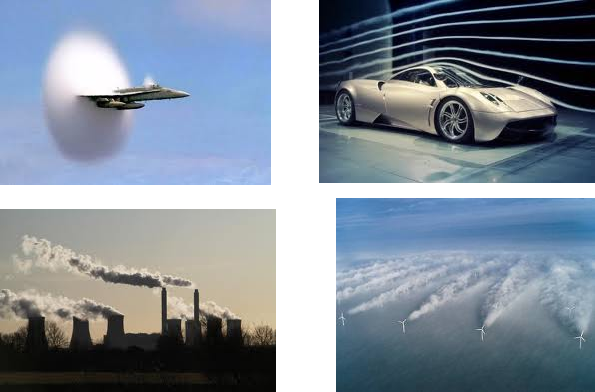
\includegraphics[width=0.9\textwidth]{hermes-motivationIn.png}
\caption{Compressible flow in nature}
\end{center}
\noindent
\vspace{-4mm}
\end{figure}
\end{frame}

\begin{frame}
\frametitle{Introduction - Compressible flow modelling}
\begin{figure}[!ht]
\vspace{-1mm}
\begin{center}
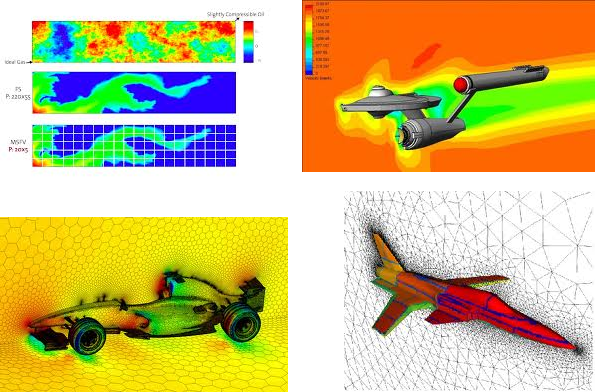
\includegraphics[width=0.9\textwidth]{hermes-motivationOut.png}
\caption{Compressible flow modelling}
\end{center}
\noindent
\vspace{-4mm}
\end{figure}
\end{frame}

\begin{frame}
\frametitle{Introduction - Hermes: numerical software}
\begin{figure}[!ht]
\vspace{-1mm}
\begin{center}
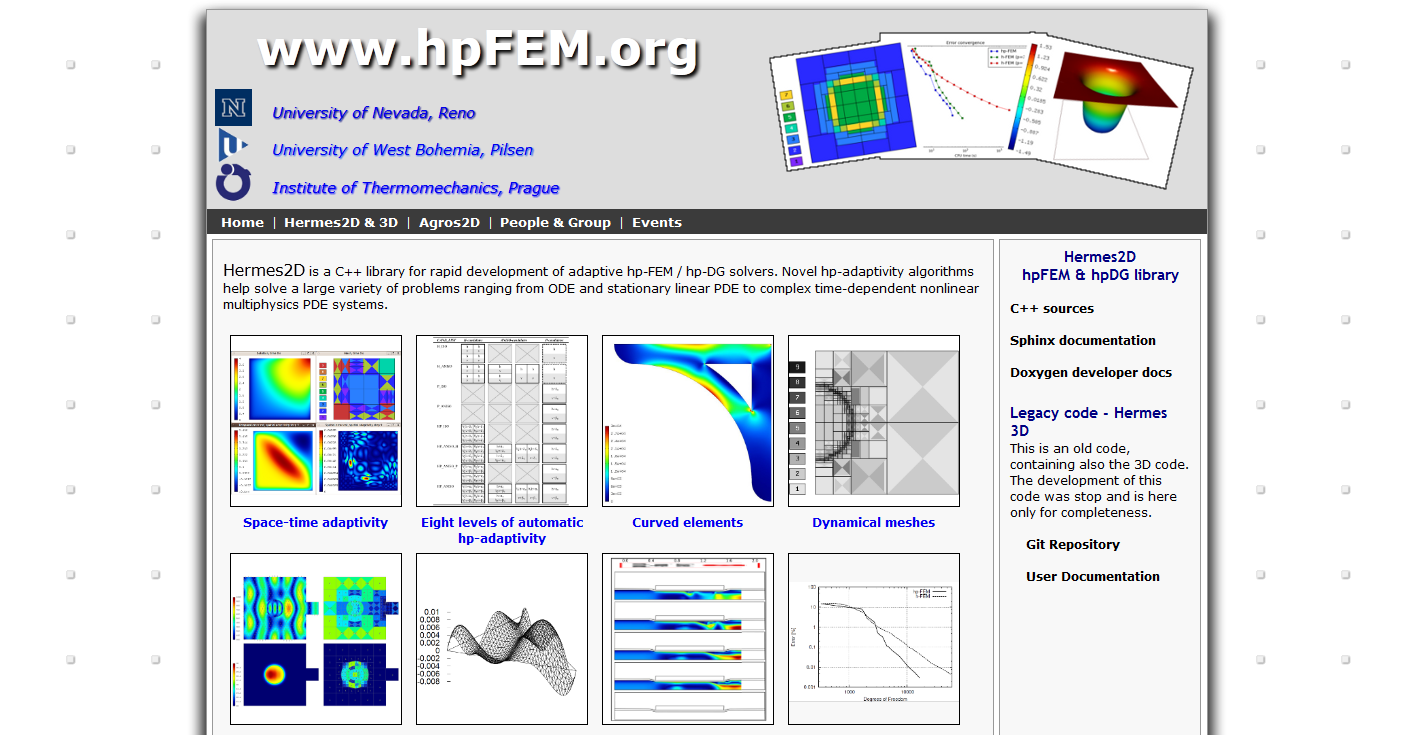
\includegraphics[width=1.0\textwidth]{hermes-site.png}
\caption{http://www.hpfem.org/hermes}
\end{center}
\noindent
\vspace{-4mm}
\end{figure}
\end{frame}

\begin{frame}
\frametitle{Introduction - Hermes}
\begin{itemize}
      \item    Unified library for handling both real and complex problems using C++ templating
      \item    Library capable of solving problems using hp-FEM and hp-DG methods and their combination
      \item    Division of the library's code into easy-to-manage namespace- and class- structure
      \item    Shared memory parallel code (using OpenMP)
      \item    XML save / load of the most important classes using provided XML schemas
      \item    Calculations with physical quantities defined in different subdomains
      \item    Exception safe API 
      \item    Supported platforms: Linux, Windows, (MAC)
      \item    Well arranged doxygen documentation
      \item    User documentation, with described examples
\end{itemize}
\end{frame}

\begin{frame}
\frametitle{Hermes: physical fields}
\begin{itemize}
      \item    Electrostatic field
      \item    Electric current field
      \item    Magnetic field
      \item    Heat transfer and Flame Propagation
      \item    Structural mechanics and Thermoelasticity
      \item    Acoustic field
      \item    Incompressible and \textbf{Compressible flow}
      \item    Advection-diffusion-reaction
      \item    Richards Equation, Wave Equation, Nernst-Planck Equation, Neutronics...
      \item    RF field: in development
\end{itemize}
\end{frame}

%Intro
\begin{frame}
\large
\frametitle{Compressible flow requirements}
In modelling of compressible flow, we would like to solve problems that\\
\begin{itemize}
\item we possess no a-priori knowledge about
\item have high Mach numbers and irregularly shaped domains
\item may have sharp discontinuities as well as smooth areas
\item may have rapidly changing solutions
\end{itemize}\ \\
Plus we would like to solve those in a reasonable time.
\end{frame}

\begin{frame}
\large
\frametitle{Compressible flow problems solutions}
\begin{itemize}
\item our discretization should be able to capture the solution
\item there should not be a need for thoroughly prepared mesh as an input
\item we should use appropriate discretization that can handle discontinuities, but which will not waste degrees of freedom for smooth areas
\item our computational mesh should evolve with the solution
\end{itemize}\ \\
All this is achieved with adaptive hp-DG method.
\end{frame}

\begin{frame}
\large
\frametitle{Numerical software internals - 1. Discretization}
\begin{figure}[!ht]
\vspace{-1mm}
\begin{center}
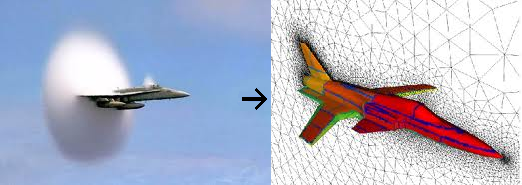
\includegraphics[width=1.0\textwidth]{Discretization.png}
\caption{Discretization}
\end{center}
\noindent
\vspace{-4mm}
\end{figure}
\end{frame}

\begin{frame}
\large
\frametitle{Numerical software internals - 1. Discretization}
\begin{figure}[!ht]
\vspace{-1mm}
\begin{center}

\includegraphics[height=0.8\textheight]{internals1.png}
\caption{Discretization}
\end{center}
\noindent
\vspace{-4mm}
\end{figure}
\end{frame}
\begin{frame}
\large
\frametitle{Numerical software internals - 1. Discretization}
\begin{figure}[!ht]
\vspace{-1mm}
\begin{center}
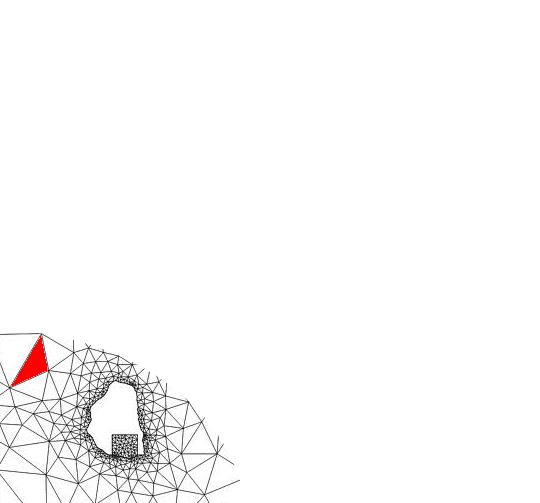
\includegraphics[height=0.8\textheight]{internals2.png}
\caption{Discretization - element}
\end{center}
\noindent
\vspace{-4mm}
\end{figure}
\end{frame}
\begin{frame}
\large
\frametitle{Numerical software internals - 2. Equations of the physical field}
\begin{figure}[!ht]
\vspace{-1mm}
\begin{center}
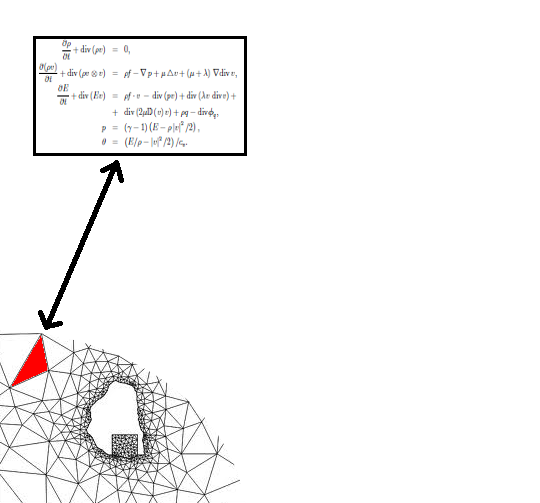
\includegraphics[height=0.8\textheight]{internals3.png}
\caption{Equations of the physical field calculated on the element}
\end{center}
\noindent
\vspace{-4mm}
\end{figure}
\end{frame}
\begin{frame}
\large
\frametitle{Numerical software internals - 2. Boundary conditions, problem data}
\begin{figure}[!ht]
\vspace{-1mm}
\begin{center}
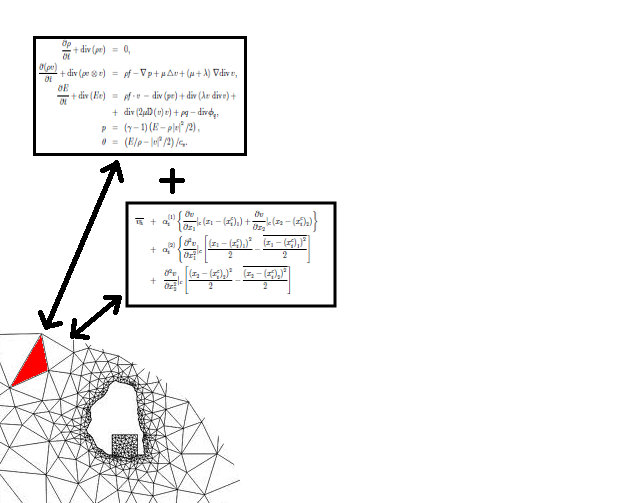
\includegraphics[height=0.8\textheight]{internals4.png}
\caption{Boundary conditions, specific data - complete the calculation on the element}
\end{center}
\noindent
\vspace{-4mm}
\end{figure}
\end{frame}
\begin{frame}
\large
\frametitle{Numerical software internals - 3. Assemble the matrix equation}
\begin{figure}[!ht]
\vspace{-1mm}
\begin{center}
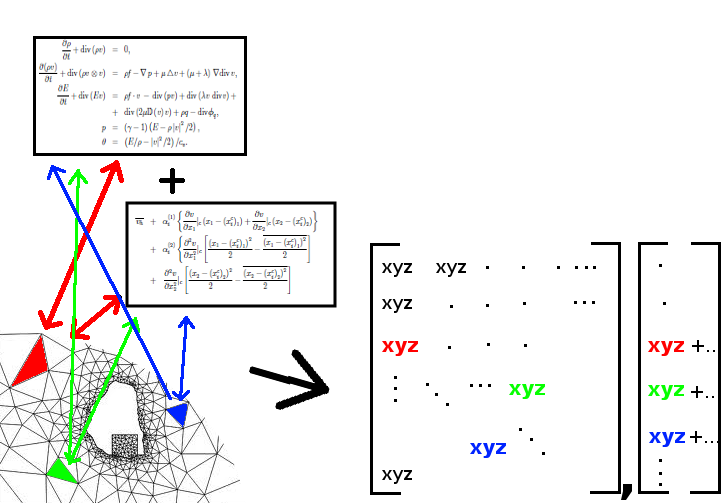
\includegraphics[height=0.8\textheight]{internals5.png}
\caption{Assemble (calculate) matrix and right-hand side entries}
\end{center}
\noindent
\vspace{-4mm}
\end{figure}
\end{frame}
\begin{frame}
\large
\frametitle{Numerical software internals - 6. Solving}
\begin{figure}[!ht]
\vspace{-1mm}
\begin{center}
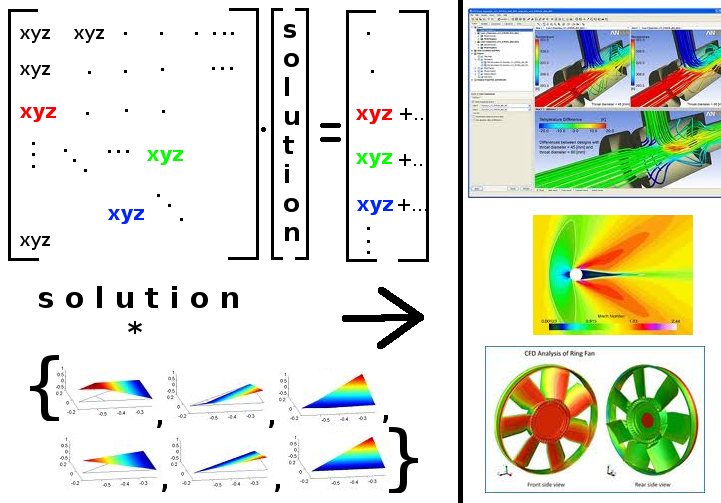
\includegraphics[height=0.8\textheight]{internals6.png}
\caption{1.Solve the matrix equation, obtain results}
\end{center}
\noindent
\vspace{-4mm}
\end{figure}
\end{frame}
\begin{frame}
\large
\frametitle{Numerical software internals - 7. Inspect results}
\begin{figure}[!ht]
\vspace{-1mm}
\begin{center}
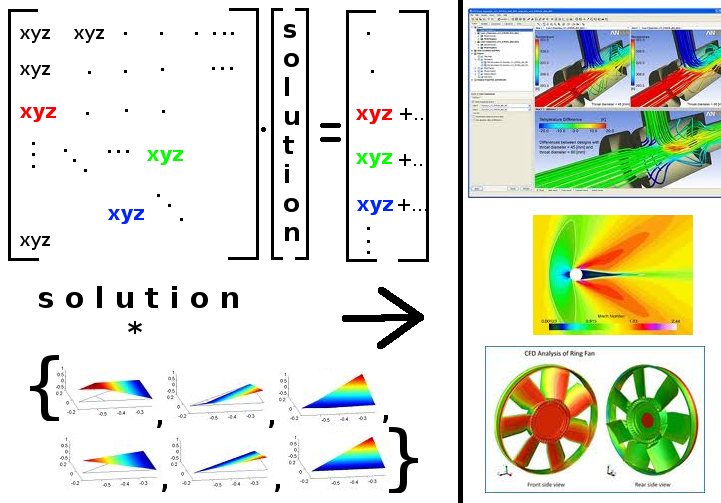
\includegraphics[height=0.8\textheight]{internals6.png}
\caption{Qualitatively and quantitatively inspect results, improve the discretization and start over if not satisfied}
\end{center}
\noindent
\vspace{-4mm}
\end{figure}
\end{frame}


\def\Tiny{\fontsize{6pt}{0pt}\selectfont}
\def\Tinya{\fontsize{8pt}{0pt}\selectfont}
\def\Tinyb{\fontsize{7pt}{0pt}\selectfont}
\definecolor{mygreen}{rgb}{0.23,0.738,0}
\begin{frame}[fragile]
\frametitle{Hermes parallel hp-FEM and hp-DG (multimesh) assembling of (nonlinear) problems}
\begin{Verbatim}[commandchars=\\\{\}, fontsize=\Tiny]
 1 \textcolor{blue}{#pragma omp parallel} shared(traverse_master, matrix, right_hand_side)
 2 num_threads(Hermes2DApi.getParamValue(Hermes::Hermes2D::numThreads))
 3 \{
 4 \textcolor{blue}{#pragma} omp for schedule(dynamic, CHUNKSIZE)
 5   \textcolor{blue}{for} (state_i = 0\textcolor{blue}{;} state_i < num_states\textcolor{blue}{;} state_i++)
 6   \{
 7 \textcolor{blue}{#pragma omp critical} (get_next_state)
 8     current_state = traverse[thread_id].get_next_state
           (&traverse_master.top, &traverse_master.id)\textcolor{blue}{;}
 9
10     basis_functions = basis_functions[thread_id]\textcolor{blue}{;}
11     test_functions = test_functions[thread_id]\textcolor{blue}{;}
12     ref_mappings = refmaps[thread_id]\textcolor{blue}{;}
13     assembly_lists = assembly_lists[thread_id]\textcolor{blue}{;}
14     forms = &(forms[thread_id].front())\textcolor{blue}{;}
15 
16     \textcolor{mygreen}{// Assemble volumetric forms and surface forms corresponding to boundary conditions.}
17     assemble_one_state(basis_functions, test_functions, ref_mappings, assembly_lists,
         &current_state, forms)\textcolor{blue}{;}
18 
19     \textcolor{mygreen}{// DG}
20     \textcolor{blue}{for} (edge = 0\textcolor{blue}{;} edge < current_state.get_number_of_edges()\textcolor{blue}{;} edge++)
21     \{
22       \textcolor{mygreen}{// Find the neighbors of this element over this edge.}
23       neighbor_groups[edge]->find_neighbors(&current_state, edge, basis_functions, 
           test_functions, ref_mappings, assembly_lists, forms)\textcolor{blue}{;}
24       
25       \textcolor{mygreen}{// Go through possibly many neighbors and assemble the forms.}
26       \textcolor{blue}{for} (neighbor = 0\textcolor{blue}{;} neighbor < neighbor_groups[edge].number_of_neighbors\textcolor{blue}{;} neighbor++)
27         neighbor_groups[edge]->assemble_one_DG_edge(neighbor)\textcolor{blue}{;}
28     \}
29   \}
30 \}
\end{Verbatim}
\end{frame}
\begin{frame}[fragile]
\frametitle{Hermes parallel hp-FEM and hp-DG (multimesh) assembling of (nonlinear) problems}
\begin{Verbatim}[commandchars=\\\{\}, fontsize=\Tiny]
 1\Tinya \textcolor{blue}{#pragma omp parallel} shared(traverse_master, matrix, right_hand_side)
 2\Tinya num_threads(Hermes2DApi.getParamValue(Hermes::Hermes2D::numThreads))
 3 \{
 4 \textcolor{blue}{#pragma} omp for schedule(dynamic, CHUNKSIZE)
 5   \textcolor{blue}{for} (state_i = 0\textcolor{blue}{;} state_i < num_states\textcolor{blue}{;} state_i++)
 6   \{
 7 \textcolor{blue}{#pragma omp critical} (get_next_state)
 8     current_state = traverse[thread_id].get_next_state
           (&traverse_master.top, &traverse_master.id)\textcolor{blue}{;}
 9
10     basis_functions = basis_functions[thread_id]\textcolor{blue}{;}
11     test_functions = test_functions[thread_id]\textcolor{blue}{;}
12     ref_mappings = refmaps[thread_id]\textcolor{blue}{;}
13     assembly_lists = assembly_lists[thread_id]\textcolor{blue}{;}
14     forms = &(forms[thread_id].front())\textcolor{blue}{;}
15 
16     \textcolor{mygreen}{// Assemble volumetric forms and surface forms corresponding to boundary conditions.}
17     assemble_one_state(basis_functions, test_functions, ref_mappings, assembly_lists,
         &current_state, forms)\textcolor{blue}{;}
18 
19     \textcolor{mygreen}{// DG}
20     \textcolor{blue}{for} (edge = 0\textcolor{blue}{;} edge < current_state.get_number_of_edges()\textcolor{blue}{;} edge++)
21     \{
22       \textcolor{mygreen}{// Find the neighbors of this element over this edge.}
23       neighbor_groups[edge]->find_neighbors(&current_state, edge, basis_functions, 
           test_functions, ref_mappings, assembly_lists, forms)\textcolor{blue}{;}
24       
25       \textcolor{mygreen}{// Go through possibly many neighbors and assemble the forms.}
26       \textcolor{blue}{for} (neighbor = 0\textcolor{blue}{;} neighbor < neighbor_groups[edge].number_of_neighbors\textcolor{blue}{;} neighbor++)
27         neighbor_groups[edge]->assemble_one_DG_edge(neighbor)\textcolor{blue}{;}
28     \}
29   \}
30 \}
\end{Verbatim}
\end{frame}
\begin{frame}[fragile]
\frametitle{Hermes parallel hp-FEM and hp-DG (multimesh) assembling of (nonlinear) problems}
\begin{Verbatim}[commandchars=\\\{\}, fontsize=\Tiny]
 1 \textcolor{blue}{#pragma omp parallel} shared(traverse_master, matrix, right_hand_side)
 2 num_threads(Hermes2DApi.getParamValue(Hermes::Hermes2D::numThreads))
 3 \{
 4 \Tinya\textcolor{blue}{#pragma} omp for schedule(dynamic, CHUNKSIZE)
 5   \Tinya\textcolor{blue}{for} (state_i = 0\textcolor{blue}{;} state_i < num_states\textcolor{blue}{;} state_i++)
 6   \{
 7 \Tinya\textcolor{blue}{#pragma omp critical} (get_next_state)
 8    \Tinya current_state = traverse[thread_id].get_next_state
           \Tinya(&traverse_master.top, &traverse_master.id)\textcolor{blue}{;}
 9
10     basis_functions = basis_functions[thread_id]\textcolor{blue}{;}
11     test_functions = test_functions[thread_id]\textcolor{blue}{;}
12     ref_mappings = refmaps[thread_id]\textcolor{blue}{;}
13     assembly_lists = assembly_lists[thread_id]\textcolor{blue}{;}
14     forms = &(forms[thread_id].front())\textcolor{blue}{;}
15 
16     \textcolor{mygreen}{// Assemble volumetric forms and surface forms corresponding to boundary conditions.}
17     assemble_one_state(basis_functions, test_functions, ref_mappings, assembly_lists,
         &current_state, forms)\textcolor{blue}{;}
18 
19     \textcolor{mygreen}{// DG}
20     \textcolor{blue}{for} (edge = 0\textcolor{blue}{;} edge < current_state.get_number_of_edges()\textcolor{blue}{;} edge++)
21     \{
22       \textcolor{mygreen}{// Find the neighbors of this element over this edge.}
23       neighbor_groups[edge]->find_neighbors(&current_state, edge, basis_functions, 
           test_functions, ref_mappings, assembly_lists, forms)\textcolor{blue}{;}
24       
25       \textcolor{mygreen}{// Go through possibly many neighbors and assemble the forms.}
26       \textcolor{blue}{for} (neighbor = 0\textcolor{blue}{;} neighbor < neighbor_groups[edge].number_of_neighbors\textcolor{blue}{;} neighbor++)
27         neighbor_groups[edge]->assemble_one_DG_edge(neighbor)\textcolor{blue}{;}
28     \}
29   \}
30 \}
\end{Verbatim}
\end{frame}
\begin{frame}[fragile]
\frametitle{Hermes parallel hp-FEM and hp-DG (multimesh) assembling of (nonlinear) problems}
\begin{Verbatim}[commandchars=\\\{\}, fontsize=\Tiny]
 1 \textcolor{blue}{#pragma omp parallel} shared(traverse_master, matrix, right_hand_side)
 2 num_threads(Hermes2DApi.getParamValue(Hermes::Hermes2D::numThreads))
 3 \{
 4 \textcolor{blue}{#pragma} omp for schedule(dynamic, CHUNKSIZE)
 5   \textcolor{blue}{for} (state_i = 0\textcolor{blue}{;} state_i < num_states\textcolor{blue}{;} state_i++)
 6   \{
 7 \textcolor{blue}{#pragma omp critical} (get_next_state)
 8     current_state = traverse[thread_id].get_next_state
           (&traverse_master.top, &traverse_master.id)\textcolor{blue}{;}
 9
10    \Tinya basis_functions = basis_functions[thread_id]\textcolor{blue}{;}
11    \Tinya test_functions = test_functions[thread_id]\textcolor{blue}{;}
12    \Tinya ref_mappings = refmaps[thread_id]\textcolor{blue}{;}
13    \Tinya assembly_lists = assembly_lists[thread_id]\textcolor{blue}{;}
14    \Tinya forms = &(forms[thread_id].front())\textcolor{blue}{;}
15 
16     \textcolor{mygreen}{// Assemble volumetric forms and surface forms corresponding to boundary conditions.}
17     assemble_one_state(basis_functions, test_functions, ref_mappings, assembly_lists,
         &current_state, forms)\textcolor{blue}{;}
18 
19     \textcolor{mygreen}{// DG}
20     \textcolor{blue}{for} (edge = 0\textcolor{blue}{;} edge < current_state.get_number_of_edges()\textcolor{blue}{;} edge++)
21     \{
22       \textcolor{mygreen}{// Find the neighbors of this element over this edge.}
23       neighbor_groups[edge]->find_neighbors(&current_state, edge, basis_functions, 
           test_functions, ref_mappings, assembly_lists, forms)\textcolor{blue}{;}
24       
25       \textcolor{mygreen}{// Go through possibly many neighbors and assemble the forms.}
26       \textcolor{blue}{for} (neighbor = 0\textcolor{blue}{;} neighbor < neighbor_groups[edge].number_of_neighbors\textcolor{blue}{;} neighbor++)
27         neighbor_groups[edge]->assemble_one_DG_edge(neighbor)\textcolor{blue}{;}
28     \}
29   \}
30 \}
\end{Verbatim}
\end{frame}
\begin{frame}[fragile]
\frametitle{Hermes parallel hp-FEM and hp-DG (multimesh) assembling of (nonlinear) problems}
\begin{Verbatim}[commandchars=\\\{\}, fontsize=\Tiny]
 1 \textcolor{blue}{#pragma omp parallel} shared(traverse_master, matrix, right_hand_side)
 2 num_threads(Hermes2DApi.getParamValue(Hermes::Hermes2D::numThreads))
 3 \{
 4 \textcolor{blue}{#pragma} omp for schedule(dynamic, CHUNKSIZE)
 5   \textcolor{blue}{for} (state_i = 0\textcolor{blue}{;} state_i < num_states\textcolor{blue}{;} state_i++)
 6   \{
 7 \textcolor{blue}{#pragma omp critical} (get_next_state)
 8     current_state = traverse[thread_id].get_next_state
           (&traverse_master.top, &traverse_master.id)\textcolor{blue}{;}
 9
10     basis_functions = basis_functions[thread_id]\textcolor{blue}{;}
11     test_functions = test_functions[thread_id]\textcolor{blue}{;}
12     ref_mappings = refmaps[thread_id]\textcolor{blue}{;}
13     assembly_lists = assembly_lists[thread_id]\textcolor{blue}{;}
14     forms = &(forms[thread_id].front())\textcolor{blue}{;}
15 
16     \textcolor{mygreen}{// Assemble volumetric forms and surface forms corresponding to boundary conditions.}
17     assemble_one_state(basis_functions, test_functions, ref_mappings, assembly_lists,
         &current_state, forms)\textcolor{blue}{;}
18 
19     \Tinya\textcolor{mygreen}{// DG}
20     \Tinya\textcolor{blue}{for} (edge = 0\textcolor{blue}{;} edge < current_state.get_number_of_edges()\textcolor{blue}{;} edge++)
21     \Tinyb\{
22       \Tinyb\textcolor{mygreen}{// Find the neighbors of this element over this edge.}
23       neighbor_groups[edge]->find_neighbors(&current_state, edge, basis_functions, 
          \Tinyb test_functions, ref_mappings, assembly_lists, forms)\textcolor{blue}{;}
24       
25       \Tinyb\textcolor{mygreen}{// Go through possibly many neighbors and assemble the forms.}
26       \textcolor{blue}{for} (neighbor = 0\textcolor{blue}{;} neighbor < neighbor_groups[edge].number_of_neighbors\textcolor{blue}{;} neighbor++)
27        \Tinyb neighbor_groups[edge]->assemble_one_DG_edge(neighbor)\textcolor{blue}{;}
28     \Tinyb\}
29   \}
30 \}
\end{Verbatim}
\end{frame}

%Adaptive mechanism
\begin{frame}
\frametitle{Hermes PDE-independent hp-adaptive algorithm for FEM}
\begin{center}
\begin{figure}[t]
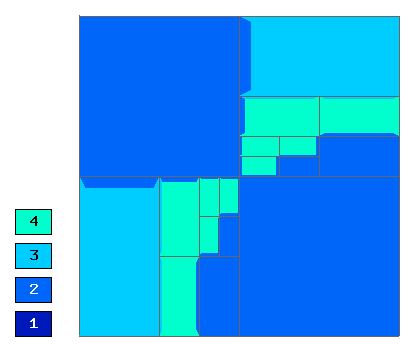
\includegraphics[width=0.42\textheight]{refsln/screen005.png}
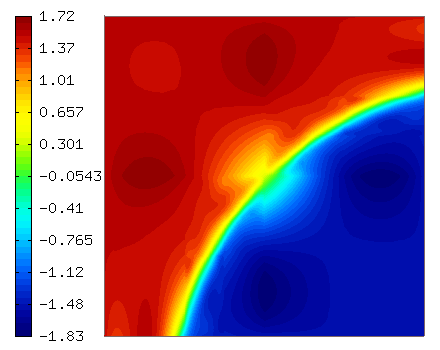
\includegraphics[width=0.42\textheight]{refsln/screen004.png}
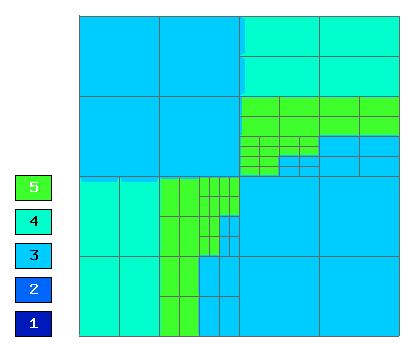
\includegraphics[width=0.42\textheight]{refsln/screen006.png}
\end{figure}
\end{center}
\vspace{43mm}
\end{frame}

%Adaptive mechanism
\begin{frame}
\frametitle{Hermes PDE-independent hp-adaptive algorithm for FEM}
\begin{center}
\begin{figure}[t]
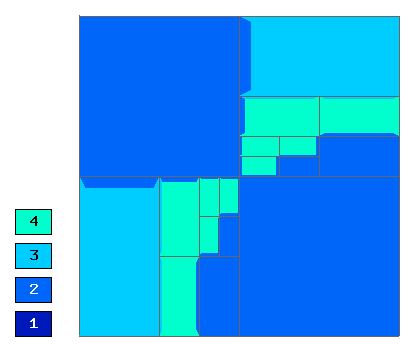
\includegraphics[width=0.42\textheight]{refsln/screen005.png}
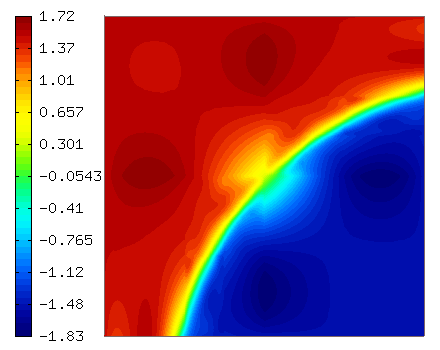
\includegraphics[width=0.42\textheight]{refsln/screen004.png}
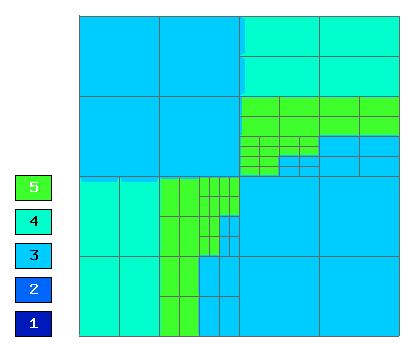
\includegraphics[width=0.42\textheight]{refsln/screen006.png}
\end{figure}
\end{center}
\begin{itemize}
\item
	By default (overridable), error estimator as a norm of the difference between the (reference) solution and the solution obtained by projection of the (reference) solution onto the \emph{coarse Space}. The formula is $Error = Norm\left(ref-coarse\right) / Norm\left(ref\right)$.
\item
	For every element, multiple refinement Candidates (h- Candidates, p- Candidates, hp- (aniso-) Candidates) are considered, and their element error is estimated using, again, local projections, but any other error estimator supplied by the user via C++ derived classes can be used.
\end{itemize}
\small
\emph{coarse Space}: The (reference) Space is actually created from this coarse Space by globally increasing polynomial degree and refining all Elements.
\end{frame}


\begin{frame}
\frametitle{Hermes PDE-independent hp-adaptive algorithm for DG}
\begin{center}
\vspace{0.86mm}
\begin{figure}[t]
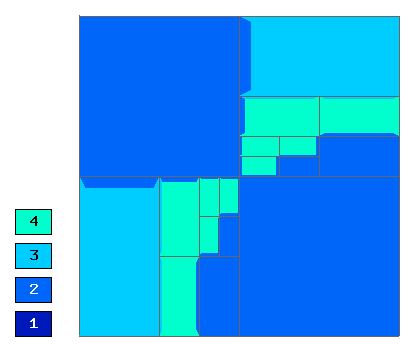
\includegraphics[width=0.42\textheight]{refsln/screen005.png}
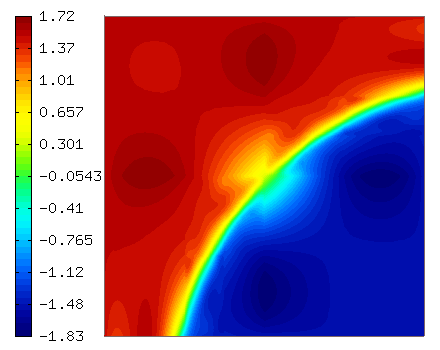
\includegraphics[width=0.42\textheight]{refsln/screen004.png}
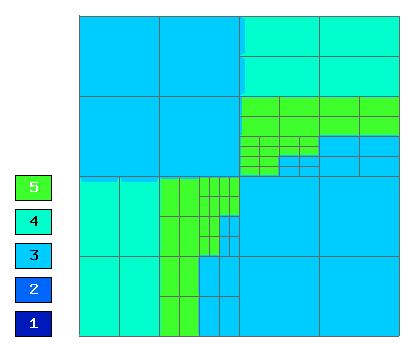
\includegraphics[width=0.42\textheight]{refsln/screen006.png}
\end{figure}
\end{center}
\vspace{-8pt}
\begin{itemize}
\item
	Error estimator based on a norm of the difference between the (reference) solution and the solution obtained by projection of the (reference) solution onto the \emph{coarse Space}. The formula is $Error = Norm\left(ref-coarse\right) / Norm\left(ref\right)$.
\item
\textcolor{red}{Suitable Shock capturing / Flux limiting method needs to be applied to the (reference) solution BEFORE projecting onto the coarse mesh, as the calculated error estimate would give incorrect results otherwise}.
\item
	For every element, multiple refinement Candidates (h- Candidates, p- Candidates, hp- (aniso-) Candidates) are considered 
(customizable by the user), and their error estimate is calculated using local projections any other error estimator supplied by the user via C++ derived classes.
\end{itemize}
\end{frame}


\begin{frame}
\frametitle{Hermes PDE-independent hp-adaptive algorithm}
\begin{center}
\vspace{0.16mm}
\begin{figure}[t]
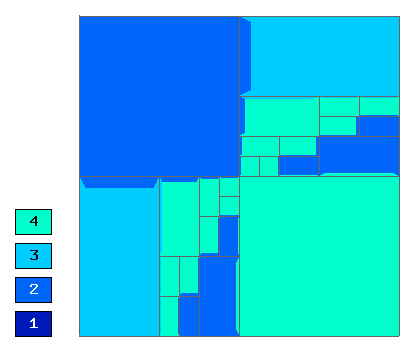
\includegraphics[width=0.42\textheight]{refsln/screen008.png}
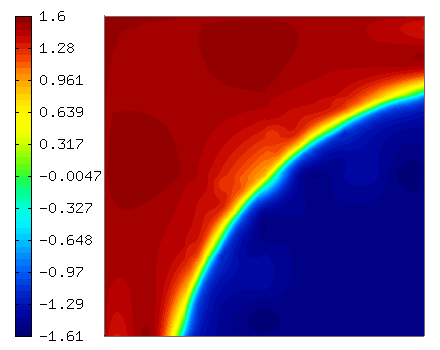
\includegraphics[width=0.42\textheight]{refsln/screen007.png}
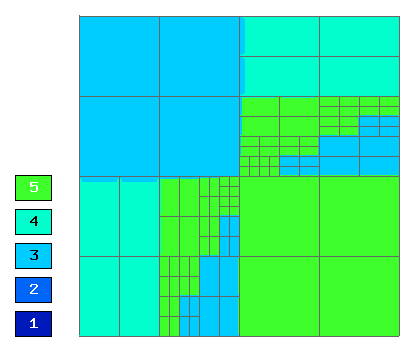
\includegraphics[width=0.42\textheight]{refsln/screen009.png}
\end{figure}
\end{center}
\begin{itemize}
\item
All Elements are initially ordered by their error estimate and they are being refined in this order unless the user does not specify otherwise.
\item
The Hermes library offers various strategies how to limit the number of refinements (amount of error processed, count of Elements refined, relative error wrt. the Element with the largest error, etc.).
\item
If an Element is chosen for refinement, the Candidate with the lowest \emph{score} is then selected and appropriate changes in Mesh and Space structures are made.
\end{itemize}
\scriptsize
\emph{score}: The number of degrees of freedom with respect to added Degrees of Freedom. The relation calculating the score is customizable using C++ derived classes from the RefinementSelector class.
\end{frame}

\begin{frame}
\frametitle{Hermes PDE-independent hp-adaptive algorithm}
\begin{center}
\vspace{0.77mm}
\begin{figure}[t]
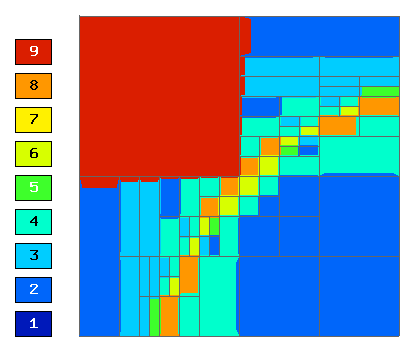
\includegraphics[width=0.42\textheight]{refsln/screen002.png}
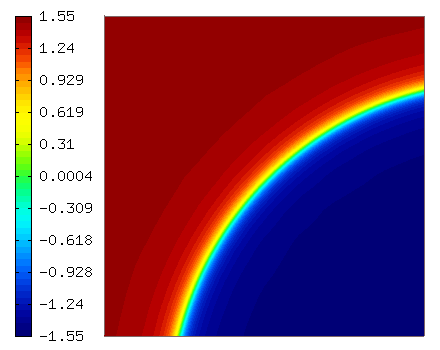
\includegraphics[width=0.42\textheight]{refsln/screen001.png}
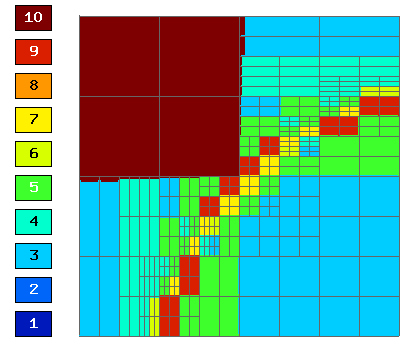
\includegraphics[width=0.42\textheight]{refsln/screen003.png}
\end{figure}
\end{center}
\begin{itemize}
\item
The refined Spaces are then used as the coarse Spaces in the next adaptivity step.
\item
The adaptivity process (at that time step) ends after a threshold for the relative difference is met, or the prescribed number of Degrees of Freedom is achieved, etc.
\item
This way (by piling up refinement layers) we would end up with unnecessarily large meshes (a lot of elements, high polynomial degrees), that is why \emph{derefinement} should be done periodically (every n-th time step):
	\begin{itemize}
	\item Decrease polynomial degree of an Element (for any set of Elements, e.g. all of them)
	\item Unrefine an Element, i.e. take out 1 level of refinement (the same)
	\item Reset the mesh completely to some base mesh.
	\end{itemize}
\end{itemize}
\end{frame}

\def\Tinyc{\fontsize{5pt}{0pt}\selectfont}
\begin{frame}[fragile]
\frametitle{Hermes PDE-independent hp-adaptive algorithm for DG}
\begin{Verbatim}[commandchars=\\\{\}, fontsize=\Tinyc]
 1 \textcolor{blue}{while}(!done)
 2 \{
 3   ref_spaces = construct_ref_spaces(&space_rho, &space_rho_v_x, &space_rho_v_y, &space_e)\textcolor{blue}{;}
 4
 5   \textcolor{mygreen}{// Uses the assembling algorithm & linear algebraic routines from TPLs.}
     \textcolor{mygreen}{// "solver" is either LinearSolver<double>, or NewtonSolver<double>, or PicardSolver<double>.}
 6   solver.solve(ref_spaces_const)\textcolor{blue}{;}
 7   
 8   \textcolor{mygreen}{// Here, the flux_limiter stands for an implementation of flux limiter,}
     \textcolor{mygreen}{// in the example that follows, limiter according to}
     \textcolor{mygreen}{// \em{D. Kuzmin.: {\em A vertex-based hierarchical slope limiter for p-adaptive discontinuous Galerkin methods}}}, 
     \textcolor{mygreen}{// \em{J. Comput. Appl. Math., \textbf{233(12)}, 3077-3085, 2010.} was used.}
 9   flux_limiter.limit_according_to_detector(&space_rho, &space_rho_v_x, &space_rho_v_y, &space_e)\textcolor{blue}{;}
10   flux_limiter.get_limited_solutions(&rsln_rho, &rsln_rho_v_x, &rsln_rho_v_y, &rsln_e)\textcolor{blue}{;}
11
12   OGProjection<double>::project_global([&space_rho, &space_rho_v_x, &space_rho_v_y, &space_e],
       [&rsln_rho, &rsln_rho_v_x, &rsln_rho_v_y, &rsln_e], [&sln_rho, &sln_rho_v_x, &sln_rho_v_y, &sln_e])\textcolor{blue}{;}
13
14   \textcolor{mygreen}{// Calculate the errors and create list of Elements accordingly.}
15   if(adaptivity->calc_error_estimate([&sln_rho, &sln_rho_v_x, &sln_rho_v_y, &sln_e],
           [&rsln_rho, &rsln_rho_v_x, &rsln_rho_v_y, &rsln_e]) < threshold) \{ done = true\textcolor{blue}{;} break\textcolor{blue}{;} \}
16 
17   \textcolor{mygreen}{// Adapt.}
18   \textcolor{blue}{#pragma} omp \textcolor{blue}{parallel} shared(...) ...
19   \{
20   \textcolor{blue}{#pragma} omp \textcolor{blue}{for} schedule(dynamic, CHUNKSIZE)
21     \textcolor{blue}{for}(element = 0\textcolor{blue}{;} element < elements.size()\textcolor{blue}{;} element++)
22     \{
23       \textcolor{blue}{if}(adaptive_strategy.done) \textcolor{blue}{break\textcolor{blue}{;}}
24       refinement_selectors = global_refinement_selectors[thread_id]\textcolor{blue}{;}
25       rslns = rslns[thread_id]\textcolor{blue}{;}
26       
27       refinement_selectors->create_candidates(element, rslns, "user settings")\textcolor{blue}{;}
28       refinement_selectors->evaluate_candidates(element, rslns, &avg_error, &dev_error)\textcolor{blue}{;}
29       refinement_selectors->select_best_candidate(element, avg_error, dev_error)\textcolor{blue}{;}
30     \}
31   \}
32   adaptivity->apply_refinements([&space_rho, &space_rho_v_x, &space_rho_v_y, &space_e])\textcolor{blue}{;}
33 \}
\end{Verbatim}
\end{frame}
\begin{frame}[fragile]
\frametitle{Hermes PDE-independent hp-adaptive algorithm for DG}
\begin{Verbatim}[commandchars=\\\{\}, fontsize=\Tinyc]
 1 \textcolor{blue}{while}(!done)
 2 \{
 3  \Tiny ref_spaces = construct_ref_spaces(&space_rho, &space_rho_v_x, &space_rho_v_y, &space_e)\textcolor{blue}{;}
 4
 5   \textcolor{mygreen}{// Uses the assembling algorithm & linear algebraic routines from TPLs.}
     \textcolor{mygreen}{// "solver" is either LinearSolver<double>, or NewtonSolver<double>, or PicardSolver<double>.}
 6   solver.solve(ref_spaces_const)\textcolor{blue}{;}
 7   
 8   \textcolor{mygreen}{// Here, the flux_limiter stands for an implementation of flux limiter,}
     \textcolor{mygreen}{// in the example that follows, limiter according to}
     \textcolor{mygreen}{// \em{D. Kuzmin.: {\em A vertex-based hierarchical slope limiter for p-adaptive discontinuous Galerkin methods}}}, 
     \textcolor{mygreen}{// \em{J. Comput. Appl. Math., \textbf{233(12)}, 3077-3085, 2010.} was used.}
 9   flux_limiter.limit_according_to_detector(&space_rho, &space_rho_v_x, &space_rho_v_y, &space_e)\textcolor{blue}{;}
10   flux_limiter.get_limited_solutions(&rsln_rho, &rsln_rho_v_x, &rsln_rho_v_y, &rsln_e)\textcolor{blue}{;}
11
12   OGProjection<double>::project_global([&space_rho, &space_rho_v_x, &space_rho_v_y, &space_e],
       [&rsln_rho, &rsln_rho_v_x, &rsln_rho_v_y, &rsln_e], [&sln_rho, &sln_rho_v_x, &sln_rho_v_y, &sln_e])\textcolor{blue}{;}
13
14   \textcolor{mygreen}{// Calculate the errors and create list of Elements accordingly.}
15   if(adaptivity->calc_error_estimate([&sln_rho, &sln_rho_v_x, &sln_rho_v_y, &sln_e],
           [&rsln_rho, &rsln_rho_v_x, &rsln_rho_v_y, &rsln_e]) < threshold) \{ done = true\textcolor{blue}{;} break\textcolor{blue}{;} \}
16 
17   \textcolor{mygreen}{// Adapt.}
18   \textcolor{blue}{#pragma} omp \textcolor{blue}{parallel} shared(...) ...
19   \{
20   \textcolor{blue}{#pragma} omp \textcolor{blue}{for} schedule(dynamic, CHUNKSIZE)
21     \textcolor{blue}{for}(element = 0\textcolor{blue}{;} element < element.size()\textcolor{blue}{;} element++)
22     \{
23       \textcolor{blue}{if}(adaptive_strategy.done) \textcolor{blue}{break\textcolor{blue}{;}}
24       refinement_selectors = global_refinement_selectors[thread_id]\textcolor{blue}{;}
25       rslns = rslns[thread_id]\textcolor{blue}{;}
26       
27       refinement_selectors->create_candidates(element, rslns, "user settings")\textcolor{blue}{;}
28       refinement_selectors->evaluate_candidates(element, rslns, &avg_error, &dev_error)\textcolor{blue}{;}
29       refinement_selectors->select_best_candidate(element, avg_error, dev_error)\textcolor{blue}{;}
30     \}
31   \}
32   adaptivity->apply_refinements([&space_rho, &space_rho_v_x, &space_rho_v_y, &space_e])\textcolor{blue}{;}
33 \}
\end{Verbatim}
\end{frame}
\begin{frame}[fragile]
\frametitle{Hermes PDE-independent hp-adaptive algorithm for DG}
\begin{Verbatim}[commandchars=\\\{\}, fontsize=\Tinyc]
 1 \textcolor{blue}{while}(!done)
 2 \{
 3   ref_spaces = construct_ref_spaces(&space_rho, &space_rho_v_x, &space_rho_v_y, &space_e)\textcolor{blue}{;}
 4
 5  \Tiny \textcolor{mygreen}{// Uses the assembling algorithm & linear algebraic routines from TPLs.}
    \Tiny \textcolor{mygreen}{// "solver" is either LinearSolver<double>, or NewtonSolver<double>, or PicardSolver<double>.}
 6  \Tiny solver.solve(ref_spaces_const)\textcolor{blue}{;}
 7   
 8   \textcolor{mygreen}{// Here, the flux_limiter stands for an implementation of flux limiter,}
     \textcolor{mygreen}{// in the example that follows, limiter according to}
     \textcolor{mygreen}{// \em{D. Kuzmin.: {\em A vertex-based hierarchical slope limiter for p-adaptive discontinuous Galerkin methods}}}, 
     \textcolor{mygreen}{// \em{J. Comput. Appl. Math., \textbf{233(12)}, 3077-3085, 2010.} was used.}
 9   flux_limiter.limit_according_to_detector(&space_rho, &space_rho_v_x, &space_rho_v_y, &space_e)\textcolor{blue}{;}
10   flux_limiter.get_limited_solutions(&rsln_rho, &rsln_rho_v_x, &rsln_rho_v_y, &rsln_e)\textcolor{blue}{;}
11
12   OGProjection<double>::project_global([&space_rho, &space_rho_v_x, &space_rho_v_y, &space_e],
       [&rsln_rho, &rsln_rho_v_x, &rsln_rho_v_y, &rsln_e], [&sln_rho, &sln_rho_v_x, &sln_rho_v_y, &sln_e])\textcolor{blue}{;}
13
14   \textcolor{mygreen}{// Calculate the errors and create list of Elements accordingly.}
15   if(adaptivity->calc_error_estimate([&sln_rho, &sln_rho_v_x, &sln_rho_v_y, &sln_e],
           [&rsln_rho, &rsln_rho_v_x, &rsln_rho_v_y, &rsln_e]) < threshold) \{ done = true\textcolor{blue}{;} break\textcolor{blue}{;} \}
16 
17   \textcolor{mygreen}{// Adapt.}
18   \textcolor{blue}{#pragma} omp \textcolor{blue}{parallel} shared(...) ...
19   \{
20   \textcolor{blue}{#pragma} omp \textcolor{blue}{for} schedule(dynamic, CHUNKSIZE)
21     \textcolor{blue}{for}(element = 0\textcolor{blue}{;} element < element.size()\textcolor{blue}{;} element++)
22     \{
23       \textcolor{blue}{if}(adaptive_strategy.done) \textcolor{blue}{break\textcolor{blue}{;}}
24       refinement_selectors = global_refinement_selectors[thread_id]\textcolor{blue}{;}
25       rslns = rslns[thread_id]\textcolor{blue}{;}
26       
27       refinement_selectors->create_candidates(element, rslns, "user settings")\textcolor{blue}{;}
28       refinement_selectors->evaluate_candidates(element, rslns, &avg_error, &dev_error)\textcolor{blue}{;}
29       refinement_selectors->select_best_candidate(element, avg_error, dev_error)\textcolor{blue}{;}
30     \}
31   \}
32   adaptivity->apply_refinements([&space_rho, &space_rho_v_x, &space_rho_v_y, &space_e])\textcolor{blue}{;}
33 \}
\end{Verbatim}
\end{frame}
\begin{frame}[fragile]
\frametitle{Hermes PDE-independent hp-adaptive algorithm for DG}
\begin{Verbatim}[commandchars=\\\{\}, fontsize=\Tinyc]
 1 \textcolor{blue}{while}(!done)
 2 \{
 3   ref_spaces = construct_ref_spaces(&space_rho, &space_rho_v_x, &space_rho_v_y, &space_e)\textcolor{blue}{;}
 4
 5   \textcolor{mygreen}{// Uses the assembling algorithm & linear algebraic routines from TPLs.}
     \textcolor{mygreen}{// "solver" is either LinearSolver<double>, or NewtonSolver<double>, or PicardSolver<double>.}
 6   solver.solve(ref_spaces_const)\textcolor{blue}{;}
 7   
 8   \Tiny\textcolor{mygreen}{// Here, the flux_limiter stands for an implementation of flux limiter,}
     \Tiny\textcolor{mygreen}{// in the example that follows, limiter according to}
     \textcolor{mygreen}{// \em{D. Kuzmin.: {\em A vertex-based hierarchical slope limiter for p-adaptive discontinuous Galerkin methods}}}, 
     \textcolor{mygreen}{// \em{J. Comput. Appl. Math., \textbf{233(12)}, 3077-3085, 2010.} was used.}
 9   flux_limiter.limit_according_to_detector(&space_rho, &space_rho_v_x, &space_rho_v_y, &space_e)\textcolor{blue}{;}
10 \Tiny flux_limiter.get_limited_solutions(&rsln_rho, &rsln_rho_v_x, &rsln_rho_v_y, &rsln_e)\textcolor{blue}{;}
11
12   OGProjection<double>::project_global([&space_rho, &space_rho_v_x, &space_rho_v_y, &space_e],
       [&rsln_rho, &rsln_rho_v_x, &rsln_rho_v_y, &rsln_e], [&sln_rho, &sln_rho_v_x, &sln_rho_v_y, &sln_e])\textcolor{blue}{;}
13
14   \textcolor{mygreen}{// Calculate the errors and create list of Elements accordingly.}
15   if(adaptivity->calc_error_estimate([&sln_rho, &sln_rho_v_x, &sln_rho_v_y, &sln_e],
           [&rsln_rho, &rsln_rho_v_x, &rsln_rho_v_y, &rsln_e]) < threshold) \{ done = true\textcolor{blue}{;} break\textcolor{blue}{;} \}
16 
17   \textcolor{mygreen}{// Adapt.}
18   \textcolor{blue}{#pragma} omp \textcolor{blue}{parallel} shared(...) ...
19   \{
20   \textcolor{blue}{#pragma} omp \textcolor{blue}{for} schedule(dynamic, CHUNKSIZE)
21     \textcolor{blue}{for}(element = 0\textcolor{blue}{;} element < element.size()\textcolor{blue}{;} element++)
22     \{
23       \textcolor{blue}{if}(adaptive_strategy.done) \textcolor{blue}{break\textcolor{blue}{;}}
24       refinement_selectors = global_refinement_selectors[thread_id]\textcolor{blue}{;}
25       rslns = rslns[thread_id]\textcolor{blue}{;}
26       
27       refinement_selectors->create_candidates(element, rslns, "user settings")\textcolor{blue}{;}
28       refinement_selectors->evaluate_candidates(element, rslns, &avg_error, &dev_error)\textcolor{blue}{;}
29       refinement_selectors->select_best_candidate(element, avg_error, dev_error)\textcolor{blue}{;}
30     \}
31   \}
32   adaptivity->apply_refinements([&space_rho, &space_rho_v_x, &space_rho_v_y, &space_e])\textcolor{blue}{;}
33 \}
\end{Verbatim}
\end{frame}
\begin{frame}[fragile]
\frametitle{Hermes PDE-independent hp-adaptive algorithm for DG}
\begin{Verbatim}[commandchars=\\\{\}, fontsize=\Tinyc]
 1 \textcolor{blue}{while}(!done)
 2 \{
 3   ref_spaces = construct_ref_spaces(&space_rho, &space_rho_v_x, &space_rho_v_y, &space_e)\textcolor{blue}{;}
 4
 5   \textcolor{mygreen}{// Uses the assembling algorithm & linear algebraic routines from TPLs.}
     \textcolor{mygreen}{// "solver" is either LinearSolver<double>, or NewtonSolver<double>, or PicardSolver<double>.}
 6   solver.solve(ref_spaces_const)\textcolor{blue}{;}
 7   
 8   \textcolor{mygreen}{// Here, the flux_limiter stands for an implementation of flux limiter,}
     \textcolor{mygreen}{// in the example that follows, limiter according to}
     \textcolor{mygreen}{// \em{D. Kuzmin.: {\em A vertex-based hierarchical slope limiter for p-adaptive discontinuous Galerkin methods}}}, 
     \textcolor{mygreen}{// \em{J. Comput. Appl. Math., \textbf{233(12)}, 3077-3085, 2010.} was used.}
 9   flux_limiter.limit_according_to_detector(&space_rho, &space_rho_v_x, &space_rho_v_y, &space_e)\textcolor{blue}{;}
10   flux_limiter.get_limited_solutions(&rsln_rho, &rsln_rho_v_x, &rsln_rho_v_y, &rsln_e)\textcolor{blue}{;}
11
12  \Tiny OGProjection<double>::project_global([&space_rho, &space_rho_v_x, &space_rho_v_y, &space_e],
       [&rsln_rho, &rsln_rho_v_x, &rsln_rho_v_y, &rsln_e], [&sln_rho, &sln_rho_v_x, &sln_rho_v_y, &sln_e])\textcolor{blue}{;}
13
14   \textcolor{mygreen}{// Calculate the errors and create list of Elements accordingly.}
15   if(adaptivity->calc_error_estimate([&sln_rho, &sln_rho_v_x, &sln_rho_v_y, &sln_e],
           [&rsln_rho, &rsln_rho_v_x, &rsln_rho_v_y, &rsln_e]) < threshold) \{ done = true\textcolor{blue}{;} break\textcolor{blue}{;} \}
16 
17   \textcolor{mygreen}{// Adapt.}
18   \textcolor{blue}{#pragma} omp \textcolor{blue}{parallel} shared(...) ...
19   \{
20   \textcolor{blue}{#pragma} omp \textcolor{blue}{for} schedule(dynamic, CHUNKSIZE)
21     \textcolor{blue}{for}(element = 0\textcolor{blue}{;} element < element.size()\textcolor{blue}{;} element++)
22     \{
23       \textcolor{blue}{if}(adaptive_strategy.done) \textcolor{blue}{break\textcolor{blue}{;}}
24       refinement_selectors = global_refinement_selectors[thread_id]\textcolor{blue}{;}
25       rslns = rslns[thread_id]\textcolor{blue}{;}
26       
27       refinement_selectors->create_candidates(element, rslns, "user settings")\textcolor{blue}{;}
28       refinement_selectors->evaluate_candidates(element, rslns, &avg_error, &dev_error)\textcolor{blue}{;}
29       refinement_selectors->select_best_candidate(element, avg_error, dev_error)\textcolor{blue}{;}
30     \}
31   \}
32   adaptivity->apply_refinements([&space_rho, &space_rho_v_x, &space_rho_v_y, &space_e])\textcolor{blue}{;}
33 \}
\end{Verbatim}
\end{frame}
\begin{frame}[fragile]
\frametitle{Hermes PDE-independent hp-adaptive algorithm for DG}
\begin{Verbatim}[commandchars=\\\{\}, fontsize=\Tinyc]
 1 \textcolor{blue}{while}(!done)
 2 \{
 3   ref_spaces = construct_ref_spaces(&space_rho, &space_rho_v_x, &space_rho_v_y, &space_e)\textcolor{blue}{;}
 4
 5   \textcolor{mygreen}{// Uses the assembling algorithm & linear algebraic routines from TPLs.}
     \textcolor{mygreen}{// "solver" is either LinearSolver<double>, or NewtonSolver<double>, or PicardSolver<double>.}
 6   solver.solve(ref_spaces_const)\textcolor{blue}{;}
 7   
 8   \textcolor{mygreen}{// Here, the flux_limiter stands for an implementation of flux limiter,}
     \textcolor{mygreen}{// in the example that follows, limiter according to}
     \textcolor{mygreen}{// \em{D. Kuzmin.: {\em A vertex-based hierarchical slope limiter for p-adaptive discontinuous Galerkin methods}}}, 
     \textcolor{mygreen}{// \em{J. Comput. Appl. Math., \textbf{233(12)}, 3077-3085, 2010.} was used.}
 9   flux_limiter.limit_according_to_detector(&space_rho, &space_rho_v_x, &space_rho_v_y, &space_e)\textcolor{blue}{;}
10   flux_limiter.get_limited_solutions(&rsln_rho, &rsln_rho_v_x, &rsln_rho_v_y, &rsln_e)\textcolor{blue}{;}
11
12   OGProjection<double>::project_global([&space_rho, &space_rho_v_x, &space_rho_v_y, &space_e],
       [&rsln_rho, &rsln_rho_v_x, &rsln_rho_v_y, &rsln_e], [&sln_rho, &sln_rho_v_x, &sln_rho_v_y, &sln_e])\textcolor{blue}{;}
13
14  \Tiny \textcolor{mygreen}{// Calculate the errors and create list of Elements accordingly.}
15  \Tiny if(adaptivity->calc_error_estimate([&sln_rho, &sln_rho_v_x, &sln_rho_v_y, &sln_e],
          [&rsln_rho, &rsln_rho_v_x, &rsln_rho_v_y, &rsln_e]) < threshold) \{ done = \Tiny true\textcolor{blue}{;} break\textcolor{blue}{;} \}
16 
17   \textcolor{mygreen}{// Adapt.}
18   \textcolor{blue}{#pragma} omp \textcolor{blue}{parallel} shared(...) ...
19   \{
20   \textcolor{blue}{#pragma} omp \textcolor{blue}{for} schedule(dynamic, CHUNKSIZE)
21     \textcolor{blue}{for}(element = 0\textcolor{blue}{;} element < elements.size()\textcolor{blue}{;} element++)
22     \{
23       \textcolor{blue}{if}(adaptive_strategy.done) \textcolor{blue}{break\textcolor{blue}{;}}
24       refinement_selectors = global_refinement_selectors[thread_id]\textcolor{blue}{;}
25       rslns = rslns[thread_id]\textcolor{blue}{;}
26       
27       refinement_selectors->create_candidates(element, rslns, "user settings")\textcolor{blue}{;}
28       refinement_selectors->evaluate_candidates(element, rslns, &avg_error, &dev_error)\textcolor{blue}{;}
29       refinement_selectors->select_best_candidate(element, avg_error, dev_error)\textcolor{blue}{;}
30     \}
31   \}
32   adaptivity->apply_refinements([&space_rho, &space_rho_v_x, &space_rho_v_y, &space_e])\textcolor{blue}{;}
33 \}
\end{Verbatim}
\end{frame}
\begin{frame}[fragile]
\frametitle{Hermes PDE-independent hp-adaptive algorithm for DG}
\begin{Verbatim}[commandchars=\\\{\}, fontsize=\Tinyc]
 1 \textcolor{blue}{while}(!done)
 2 \{
 3   ref_spaces = construct_ref_spaces(&space_rho, &space_rho_v_x, &space_rho_v_y, &space_e)\textcolor{blue}{;}
 4
 5   \textcolor{mygreen}{// Uses the assembling algorithm & linear algebraic routines from TPLs.}
     \textcolor{mygreen}{// "solver" is either LinearSolver<double>, or NewtonSolver<double>, or PicardSolver<double>.}
 6   solver.solve(ref_spaces_const)\textcolor{blue}{;}
 7   
 8   \textcolor{mygreen}{// Here, the flux_limiter stands for an implementation of flux limiter,}
     \textcolor{mygreen}{// in the example that follows, limiter according to}
     \textcolor{mygreen}{// \em{D. Kuzmin.: {\em A vertex-based hierarchical slope limiter for p-adaptive discontinuous Galerkin methods}}}, 
     \textcolor{mygreen}{// \em{J. Comput. Appl. Math., \textbf{233(12)}, 3077-3085, 2010.} was used.}
 9   flux_limiter.limit_according_to_detector(&space_rho, &space_rho_v_x, &space_rho_v_y, &space_e)\textcolor{blue}{;}
10   flux_limiter.get_limited_solutions(&rsln_rho, &rsln_rho_v_x, &rsln_rho_v_y, &rsln_e)\textcolor{blue}{;}
11
12   OGProjection<double>::project_global([&space_rho, &space_rho_v_x, &space_rho_v_y, &space_e],
       [&rsln_rho, &rsln_rho_v_x, &rsln_rho_v_y, &rsln_e], [&sln_rho, &sln_rho_v_x, &sln_rho_v_y, &sln_e])\textcolor{blue}{;}
13
14   \textcolor{mygreen}{// Calculate the errors and create list of Elements accordingly.}
15   if(adaptivity->calc_error_estimate([&sln_rho, &sln_rho_v_x, &sln_rho_v_y, &sln_e],
           [&rsln_rho, &rsln_rho_v_x, &rsln_rho_v_y, &rsln_e]) < threshold) \{ done = true\textcolor{blue}{;} break\textcolor{blue}{;} \}
16 
17  \Tiny \textcolor{mygreen}{// Adapt.}
18  \Tiny \textcolor{blue}{#pragma} omp \textcolor{blue}{parallel} shared(...) ...
19  \Tiny \{
20  \Tiny \textcolor{blue}{#pragma} omp \textcolor{blue}{for} schedule(dynamic, CHUNKSIZE)
21    \Tiny \textcolor{blue}{for}(element = 0\textcolor{blue}{;} element < element.size()\textcolor{blue}{;} element++)
22    \Tiny \{
23      \Tiny \textcolor{blue}{if}(adaptive_strategy.done) \textcolor{blue}{break\textcolor{blue}{;}}
24     \Tiny  refinement_selectors = global_refinement_selectors[thread_id]\textcolor{blue}{;}
25     \Tiny  rslns = rslns[thread_id]\textcolor{blue}{;}
26       
27     \Tiny  refinement_selectors->create_candidates(element, rslns, "user settings")\textcolor{blue}{;}
28    \Tiny   refinement_selectors->evaluate_candidates(element, rslns, &avg_error, &dev_error)\textcolor{blue}{;}
29    \Tiny   refinement_selectors->select_best_candidate(element, avg_error, dev_error)\textcolor{blue}{;}
30   \Tiny  \}
31  \Tiny \}
32 \Tiny  adaptivity->apply_refinements([&space_rho, &space_rho_v_x, &space_rho_v_y, &space_e])\textcolor{blue}{;}
33 \}
\end{Verbatim}
\end{frame}


%Discretization
\begin{frame}
\frametitle{Discretization of time dependent problems}
Rothe's method and dynamical meshes
\begin{itemize}
\item discretization in time first
\item discretized problem at each time level solved by adaptive hp-DG
\item meshes evolve in time independently of each other (common original mesh)
\end{itemize}
\begin{center}
\includegraphics[width=0.5\textwidth]{shot0001.png}
\end{center}
\end{frame}
%Discretization
\begin{frame}
\frametitle{Discretization of time dependent problems}
Rothe's method and dynamical meshes
\begin{itemize}
\item discretization in time first
\item discretized problem at each time level solved by adaptive hp-DG
\item meshes evolve in time independently of each other (common original mesh)
\end{itemize}
\begin{center}
\includegraphics[width=0.5\textwidth]{shot0002.png}
\end{center}
\end{frame}%Discretization
\begin{frame}
\frametitle{Discretization of time dependent problems}
Rothe's method and dynamical meshes
\begin{itemize}
\item discretization in time first
\item discretized problem at each time level solved by adaptive hp-DG
\item meshes evolve in time independently of each other (common original mesh)
\end{itemize}
\begin{center}
\includegraphics[width=0.5\textwidth]{shot0003.png}
\end{center}
\end{frame}%Discretization
\begin{frame}
\frametitle{Discretization of time dependent problems}
Rothe's method and dynamical meshes
\begin{itemize}
\item discretization in time first
\item discretized problem at each time level solved by adaptive hp-DG
\item meshes evolve in time independently of each other (common original mesh)
\end{itemize}
\begin{center}
\includegraphics[width=0.5\textwidth]{shot0004.png}
\end{center}
\end{frame}
\begin{frame}
\frametitle{Discretization of time dependent problems}
Rothe's method and dynamical meshes
\begin{itemize}
\item discretization in time first
\item discretized problem at each time level solved by adaptive hp-DG
\item meshes evolve in time independently of each other (common original mesh)
\end{itemize}
\begin{center}
\includegraphics[width=0.5\textwidth]{shot0005.png}
\end{center}
\end{frame}

\begin{frame}
 \frametitle{Numerical example - flow around a Joukowski profile}
	Benchmark: Subsonic flow around airfoil.
\begin{center}
$$\movie[width=0.9\textwidth]{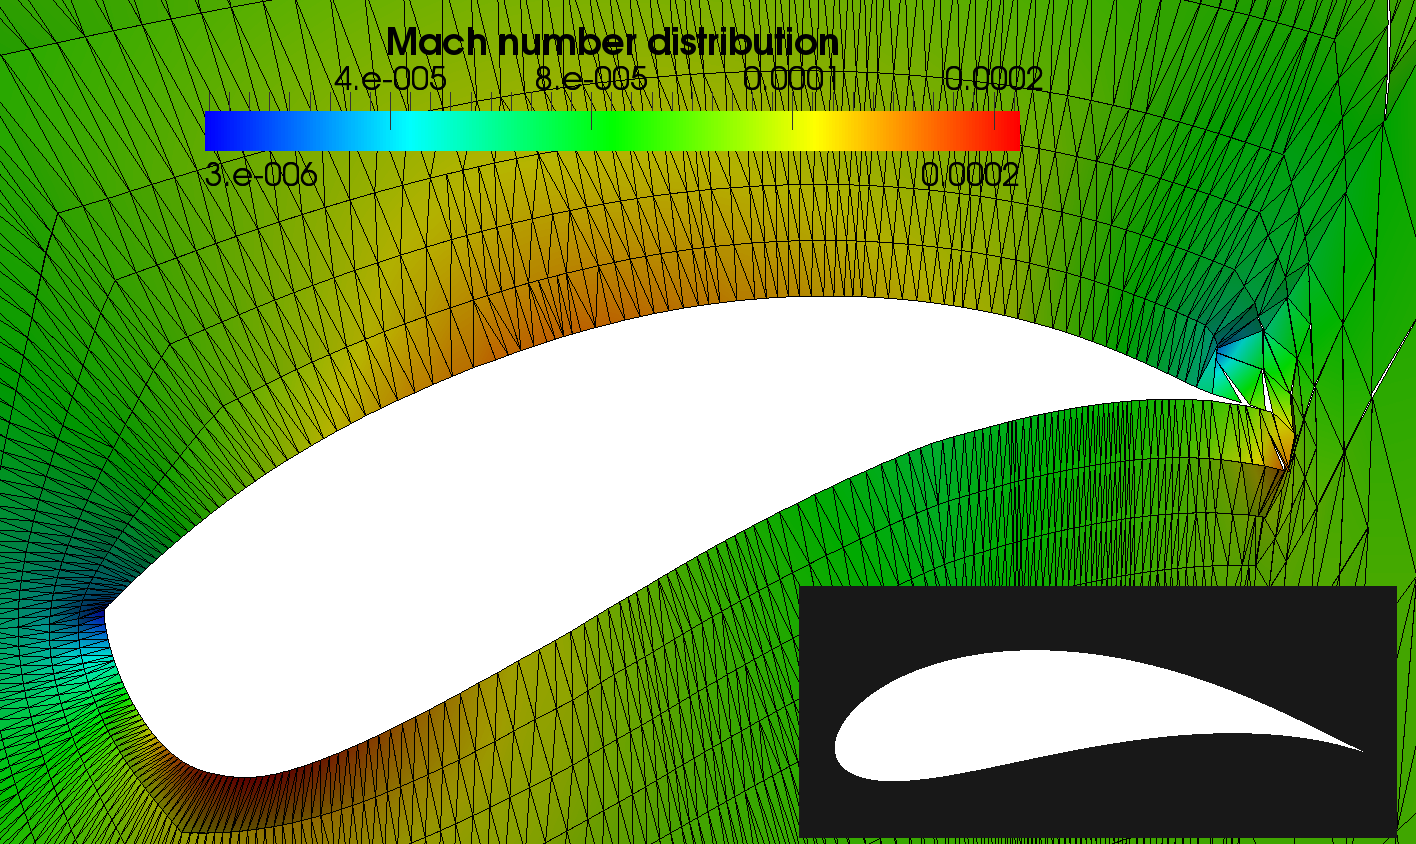
\includegraphics[width=0.9\textwidth]{output1.png}}{jouk.avi}$$
\end{center}
\end{frame}

\begin{frame}
 \frametitle{Numerical example - channel with a bump}
	A supersonic flows hits a bump in a channel and produces a shockwave.
$$\movie[width=\textwidth,height=0.6\textwidth]{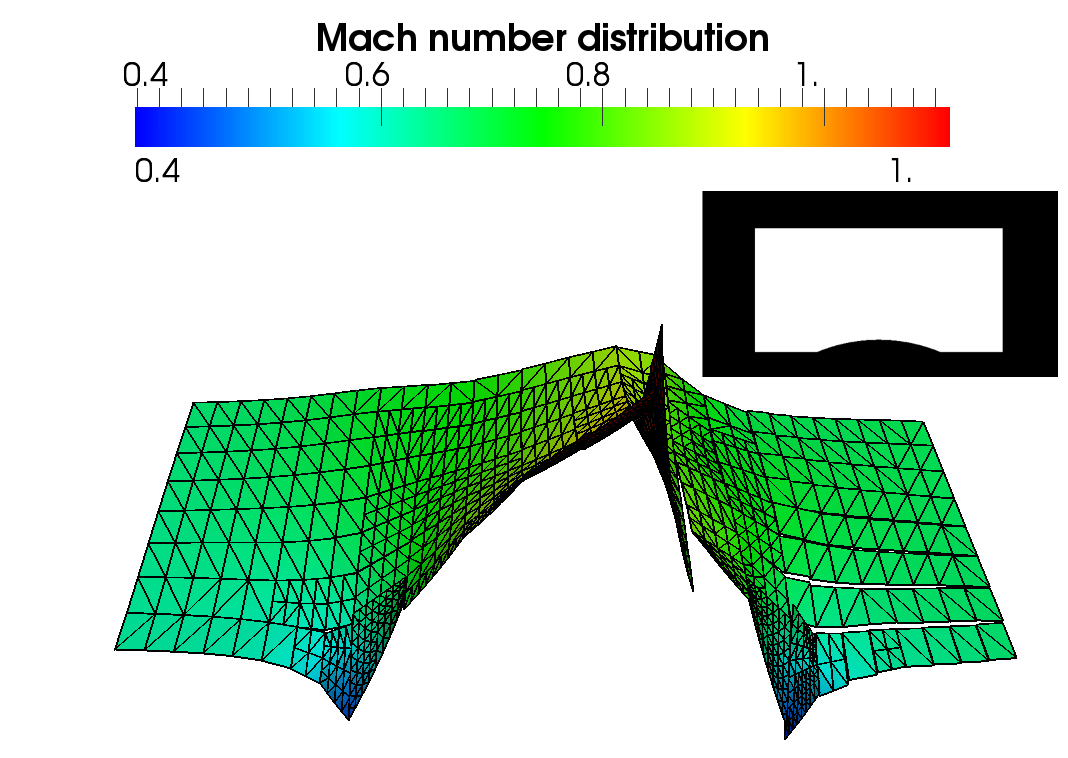
\includegraphics[width=\textwidth,height=0.6\textwidth]{output2.png}}{gamm-new.avi}$$
\end{frame}


\begin{frame}
 \frametitle{Numerical example - reflected shock}
	Benchmark: Two supersonic flows meeting and reflecting off a wall.\\
	Known exact solution.
\begin{center}
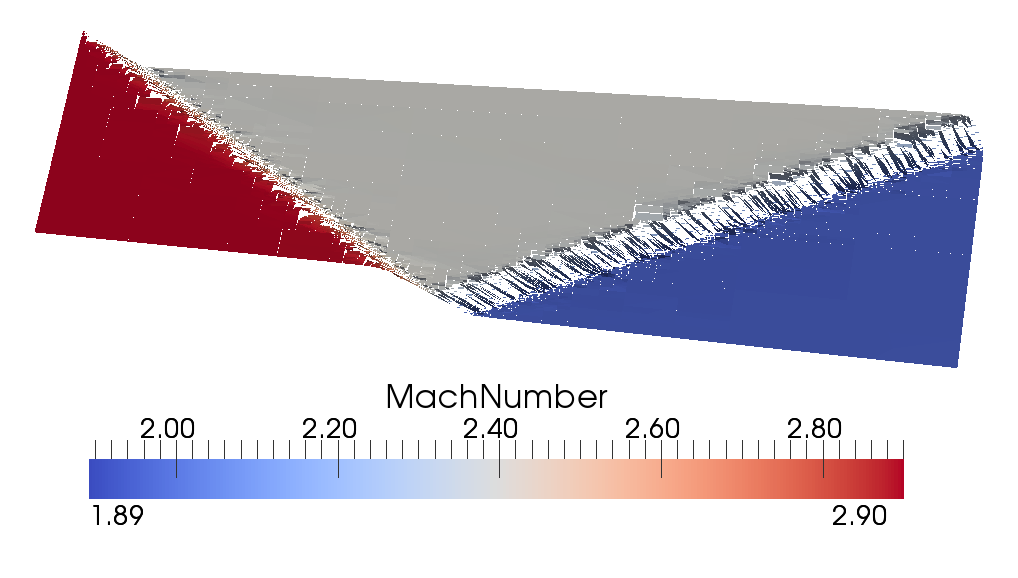
\includegraphics[width=\textwidth]{refl/screen.png}
\end{center}
\end{frame}

\begin{frame}
 \frametitle{Numerical example - reflected shock}
	Benchmark: Two supersonic flows meeting and reflecting off a wall.\\
	Known exact solution.
\begin{center}
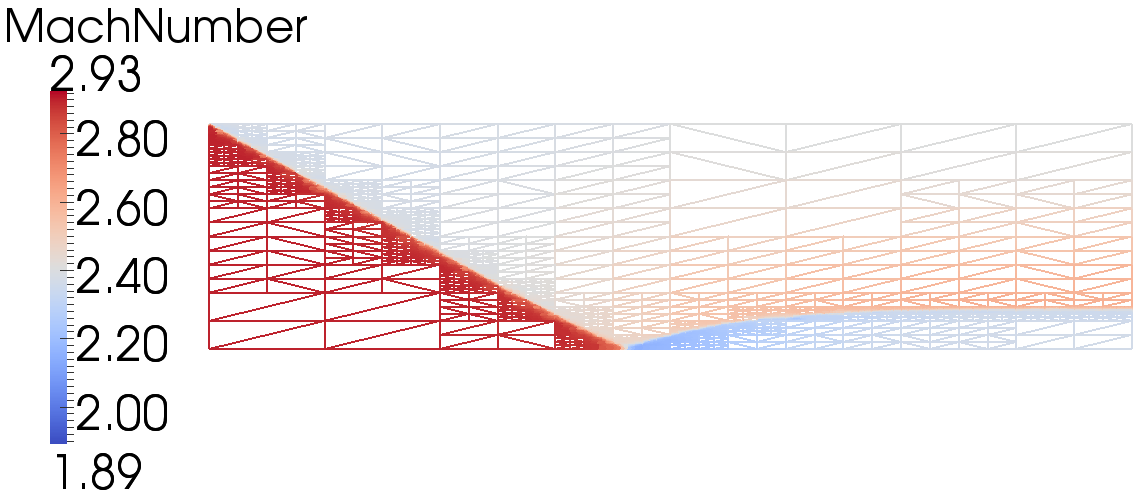
\includegraphics[width=0.75\textwidth]{refl/screen01-sln.png}\\
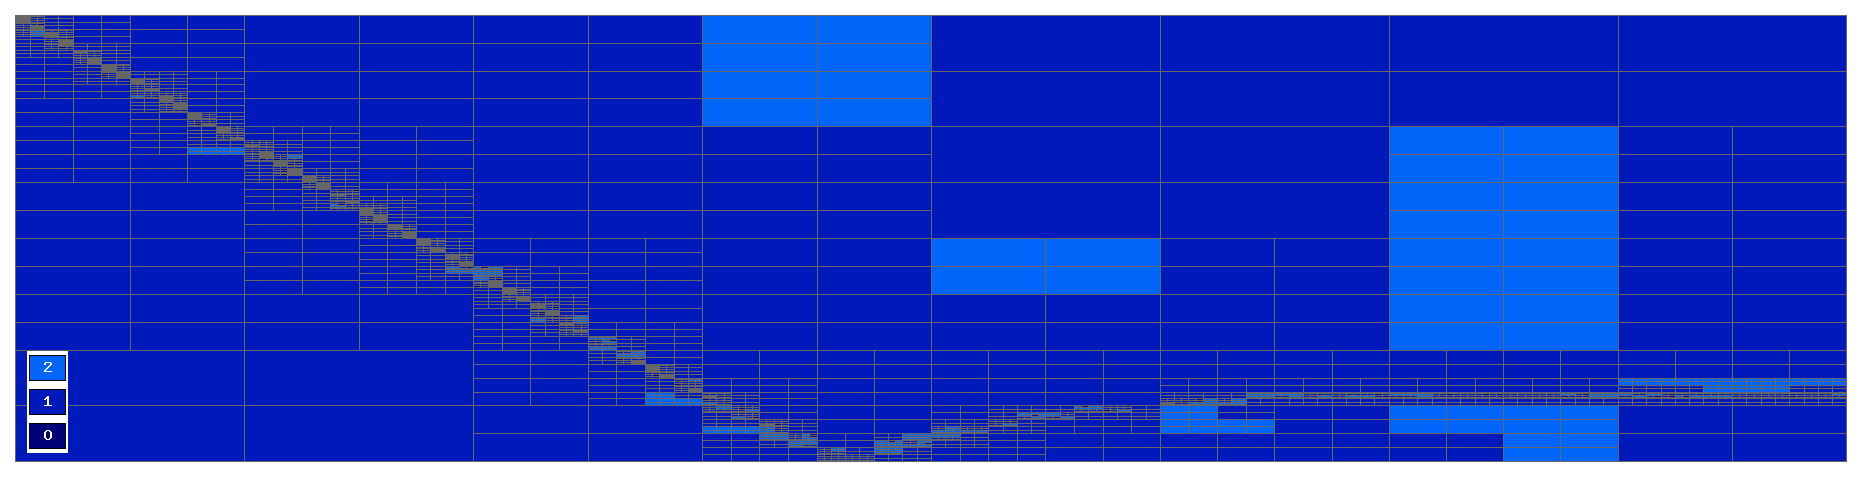
\includegraphics[width=0.75\textwidth]{refl/screen001whole.png}
\end{center}
\end{frame}

\begin{frame}
 \frametitle{Numerical example - reflected shock}
	Benchmark: Two supersonic flows meeting and reflecting off a wall.\\
	Known exact solution.
\begin{center}
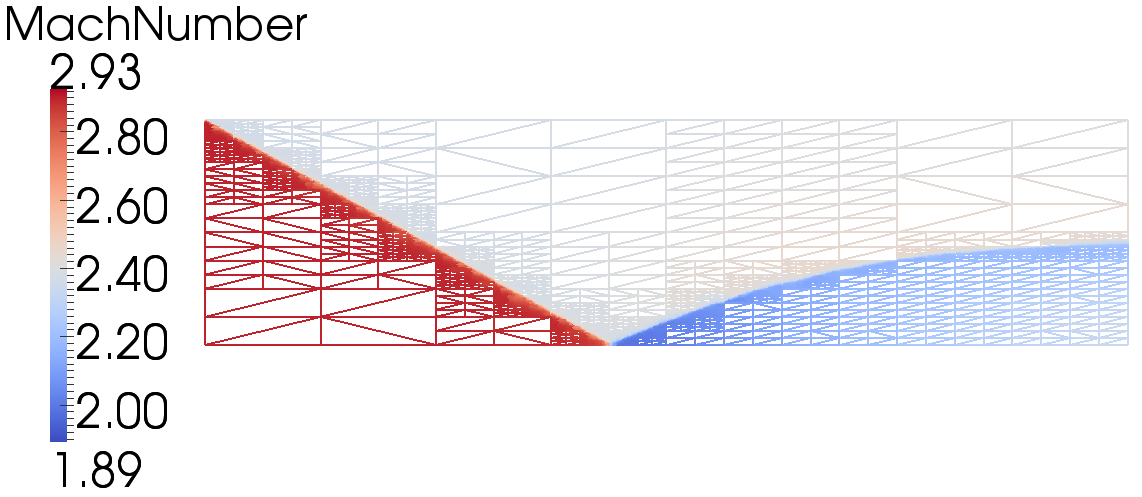
\includegraphics[width=0.75\textwidth]{refl/screen02-sln.png}\\
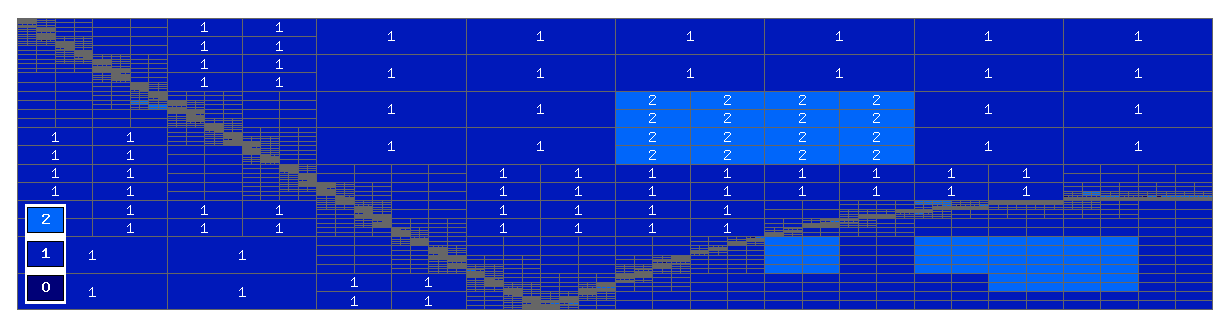
\includegraphics[width=0.75\textwidth]{refl/screen002whole.png}
\end{center}
\end{frame}

\begin{frame}
 \frametitle{Numerical example - reflected shock}
	Benchmark: Two supersonic flows meeting and reflecting off a wall.\\
	Known exact solution.
\begin{center}
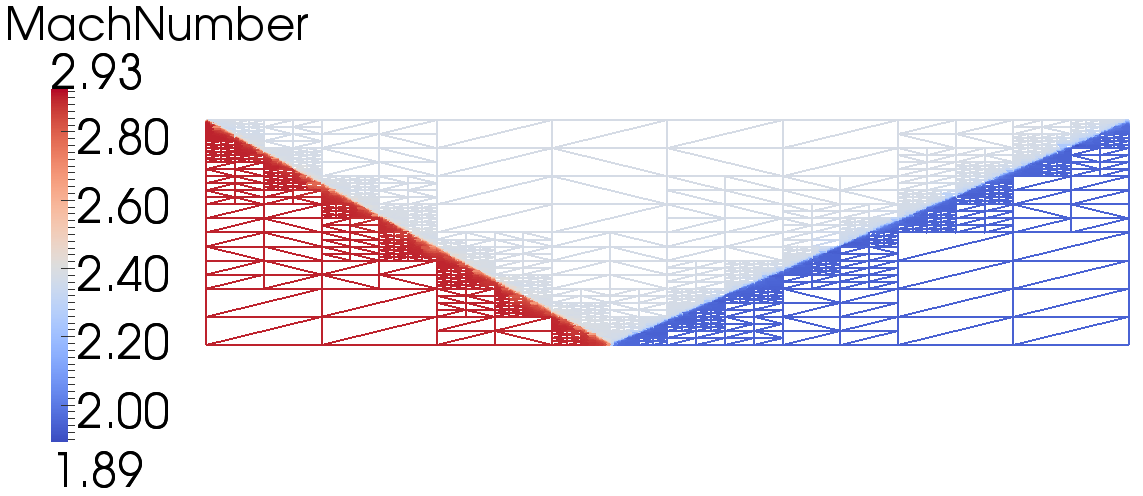
\includegraphics[width=0.75\textwidth]{refl/screen03-sln.png}\\
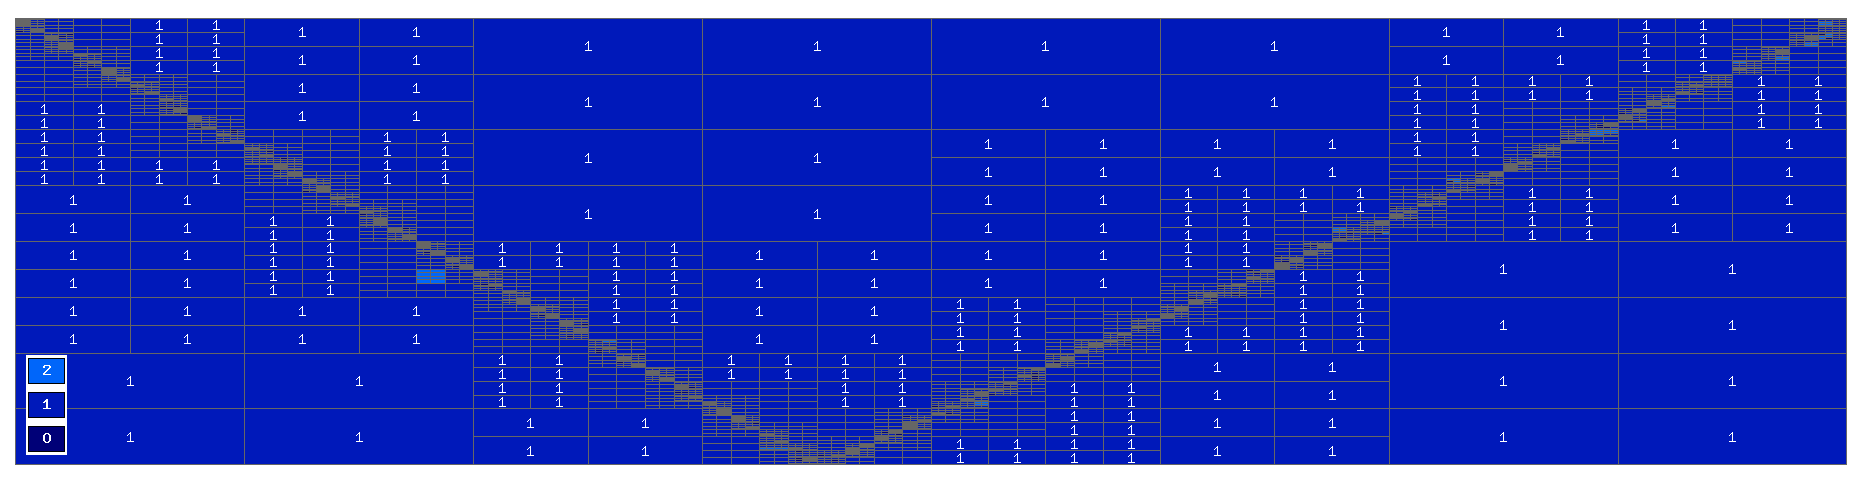
\includegraphics[width=0.75\textwidth]{refl/screen003whole.png}
\end{center}
\end{frame}

\begin{frame}
 \frametitle{Numerical example - reflected shock}
	Two supersonic flows meeting and reflecting off a wall.\\
	Known exact solution.
$$\movie[width=\textwidth,height=0.6\textwidth]{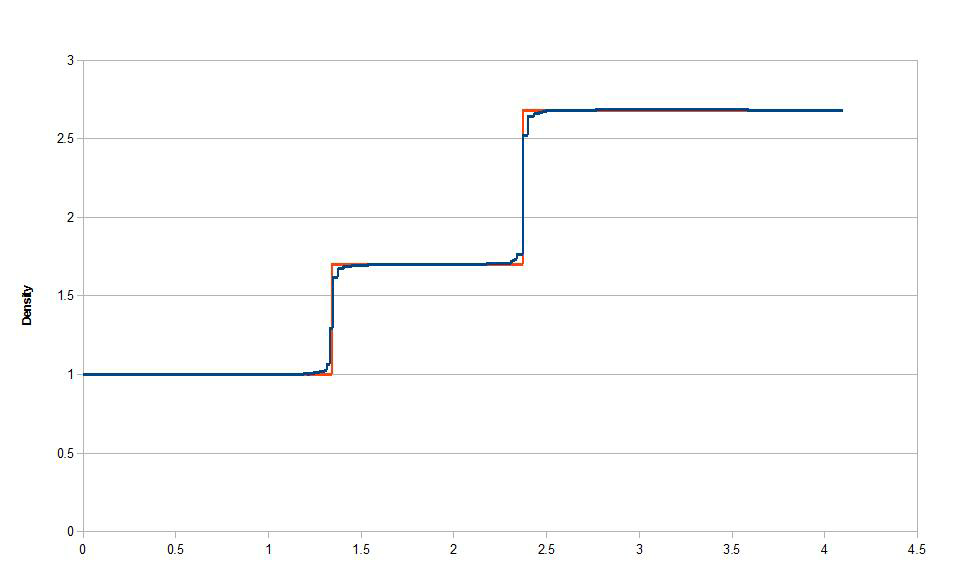
\includegraphics[width=\textwidth,height=0.6\textwidth]{refl/density.png}}{refl/reflected-shock.avi}$$
\end{frame}

\begin{frame}
\frametitle{Outlook}
Outlook:
\begin{itemize}
\item coupling with other physical fields (work in progress)
\item similar capabilities in 3D
\item More complicated geometries
\item Domain decomposition, MPI, multi- (many-) node parallelization
\end{itemize}
\end{frame}

\begin{frame}
\frametitle{The End}
\begin{center}
\LARGE
Thank you for your kind attention.
\end{center}
\end{frame}


\end{document}
